% \documentclass[a4]{scrartcl}

\documentclass[12pt,a4paper, usenames, dvipsnames]{scrartcl}
\usepackage{graphicx}
\usepackage{xcolor}


\usepackage[ngerman]{babel}
\usepackage[utf8]{inputenc}
\usepackage{mathtools}
\usepackage{amsmath}
\usepackage{amssymb}
\usepackage{geometry}
\usepackage{scrpage2}
\usepackage{tikz}
\usepackage{verbatim}

\usepackage{subfigure}
\usepackage[center]{caption}


\pagestyle{plain}
% \clearscrheadfoot
\pagenumbering {arabic} 

\usepackage[backend=bibtex,style=numeric, citestyle = numeric]{biblatex}
\addbibresource{quellen.bib}

\usepackage[babel,german=guillemets]{csquotes}




\geometry{
  paper=a4paper, % Change to letterpaper for US letter
  top=1.5cm, % Top margin
  left=2cm, % Left margin
  right=3cm, % Right margin
  %showframe, % Uncomment to show how the type block is set on the page
}

\pagenumbering {arabic} 









\begin{document}



\begin{titlepage}
	\centering
	\vspace*{4cm}
	{\scshape\LARGE Technische Universität Dortmund \par}
	\vspace{1cm}
	{\scshape\Large Proposal \\
	(zur Bachelorarbeit) \par}
	\vspace{1.5cm}
	{\huge\bfseries Zauberwürfel Algorithmen und deren Tiefe an einem 2x2x2 Würfel\par}
	\vspace{2cm}
	{\Large\itshape Pina Kolling\par}
	\vfill
	betreut von\par
	Dr. Lukasz \textsc{Czajka}

	\vfill

% Bottom of the page
	{\large \today\par}
\end{titlepage}


\tableofcontents

\thispagestyle{empty} 



\newpage

\setcounter{page}{1} 

\section{Einleitung/Ausgangslage}

Meine Bachelorarbeit soll sich mit dem 2x2x2 Zauberwürfel und dessen Algorithmen zur Lösung befassen. Dabei handelt es sich um ein Drehpuzzle, das ein mathematisches Problem darstellt. \\ 
Ich möchte sowohl die Algorithmen mithilfe der Gruppentheorie darstellen, als auch einen Code zur Berechnung der tiefsten Tiefe (Definition der Tiefe folgt) schreiben als auch die 3x3x3 Algorithmen auf den 2x2x2 Würfel übertragen. \\
Im folgenden werde ich die Terminologie und des Aufbau des Würfels klären.\\
Terminologie:
\begin{figure}[h]
\centering
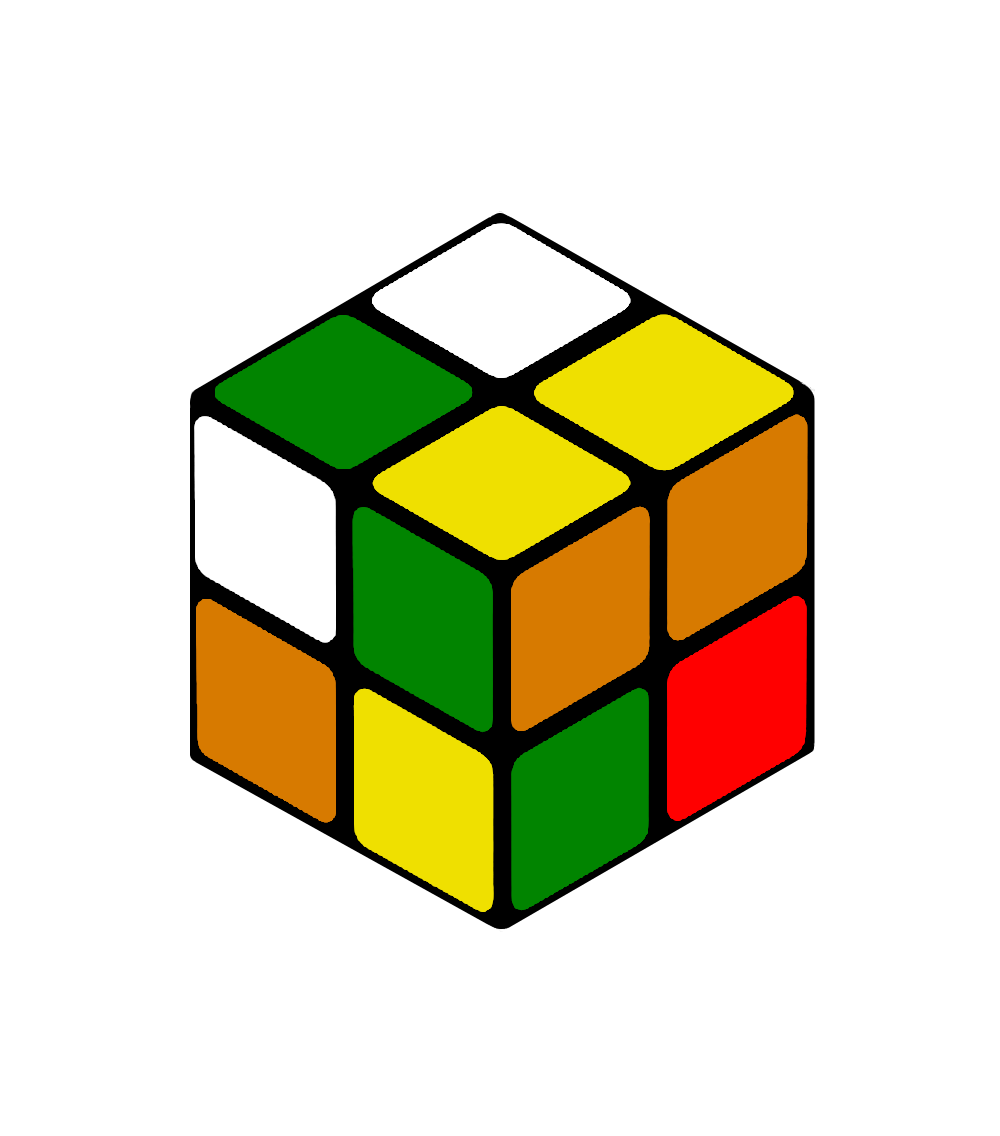
\includegraphics[scale=0.1]{2x2scrambled.png}
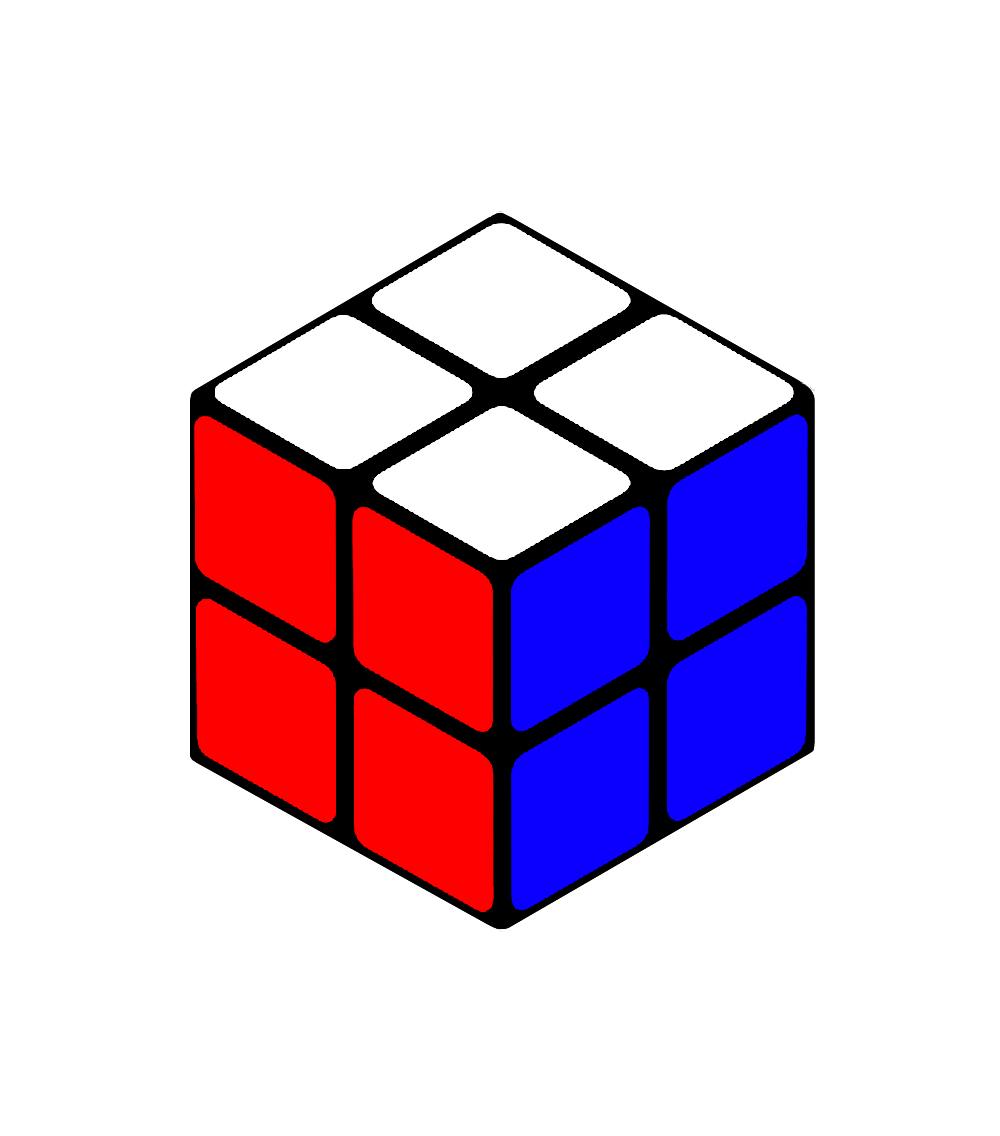
\includegraphics[scale=0.1]{2x2solved.png}
\caption{2x2x2 Zauberwürfel \\ (links in ungelöstem und rechts in gelöstem Zustand (auch Grundstellung)) \\
Der Zauberwürfel wird auch Würfel/Cube genannt.}
\end{figure}

\begin{figure}[h]
\centering
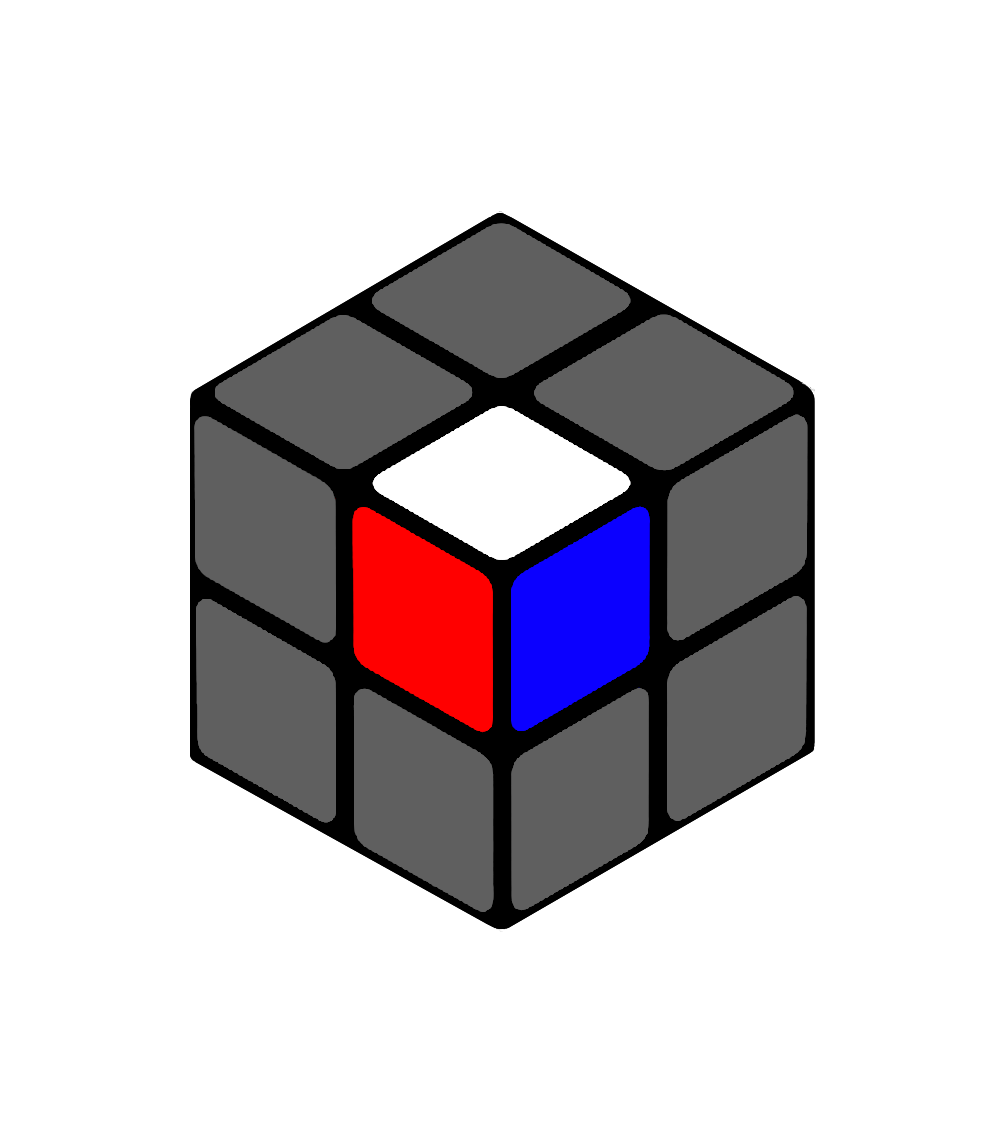
\includegraphics[scale=0.1]{2x2stein.png}
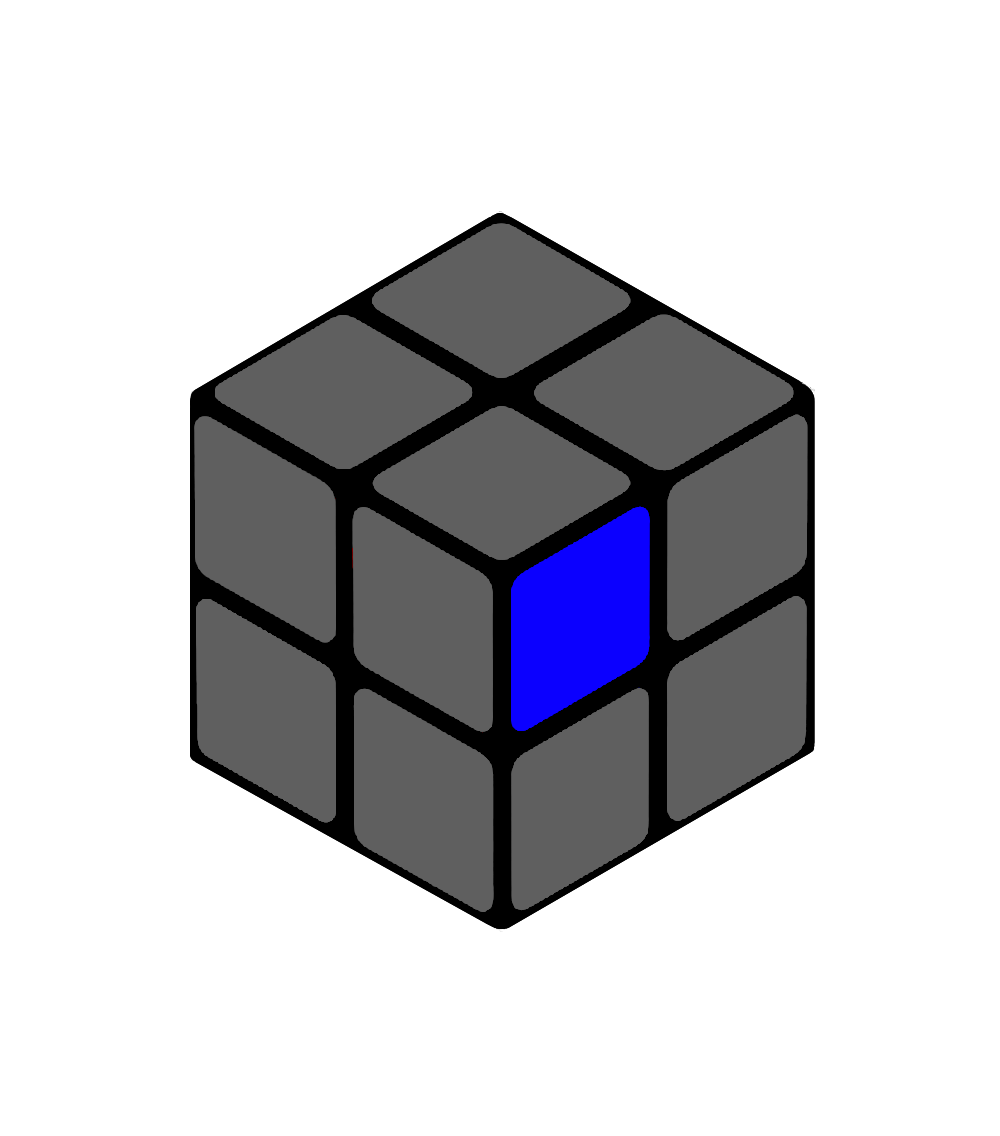
\includegraphics[scale=0.1]{2x2farbflaeche.png}
\caption{Ein 2x2x2 Würfel besteht aus 8 (Eck-)Steinen (links), die jeweils 3 Farbflächen (rechts) haben. Ein 2x2x2 Zauberwürfel hat also 24 Farbflächen.}
\end{figure}

\begin{figure}[h]
\centering
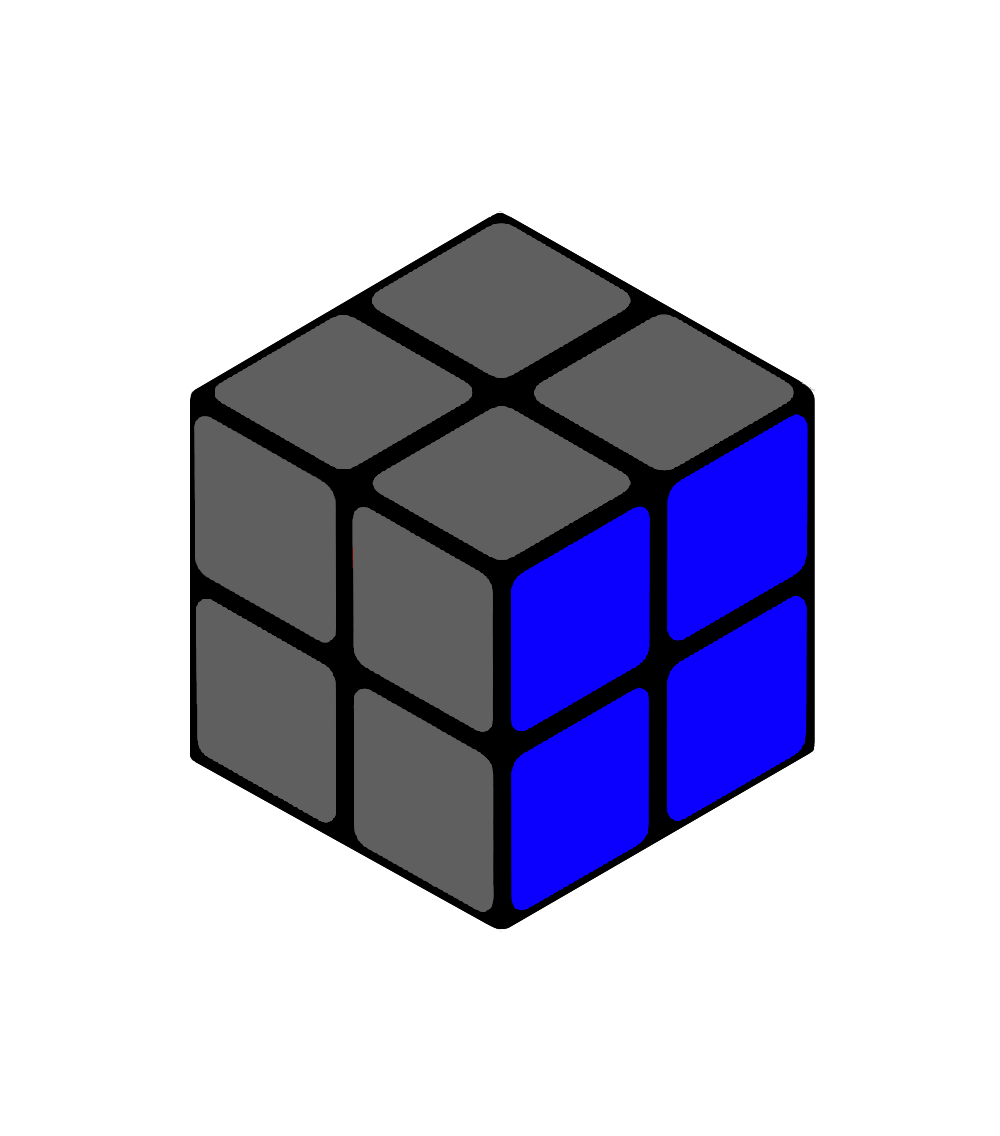
\includegraphics[scale=0.1]{2x2seite.png}
\caption{Der 2x2x2 und der 3x3x3 Zauberwürfel haben jeweils 6 Seiten.}
\end{figure}

\newpage


\begin{figure}[h]
\centering
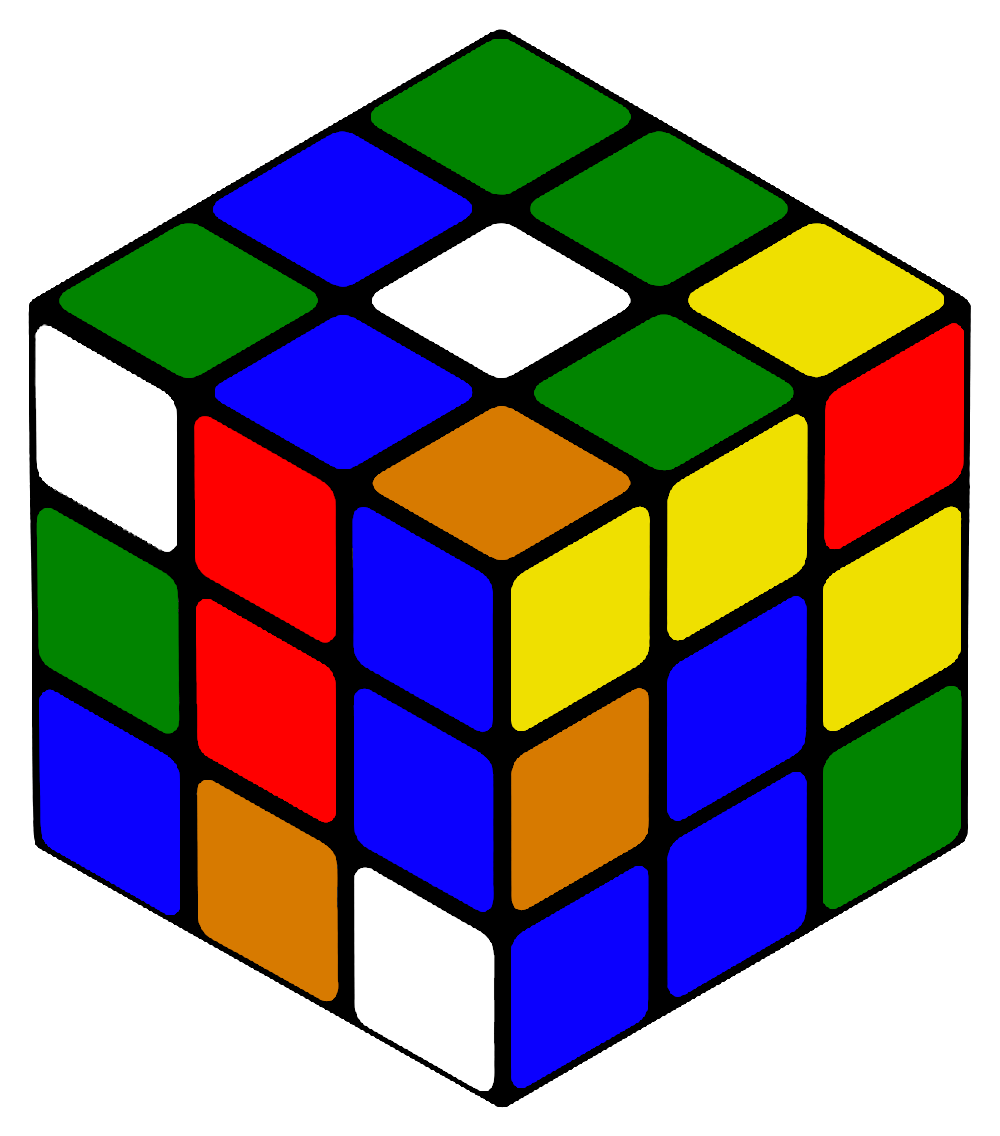
\includegraphics[scale=0.09]{3x3scrambled.png}
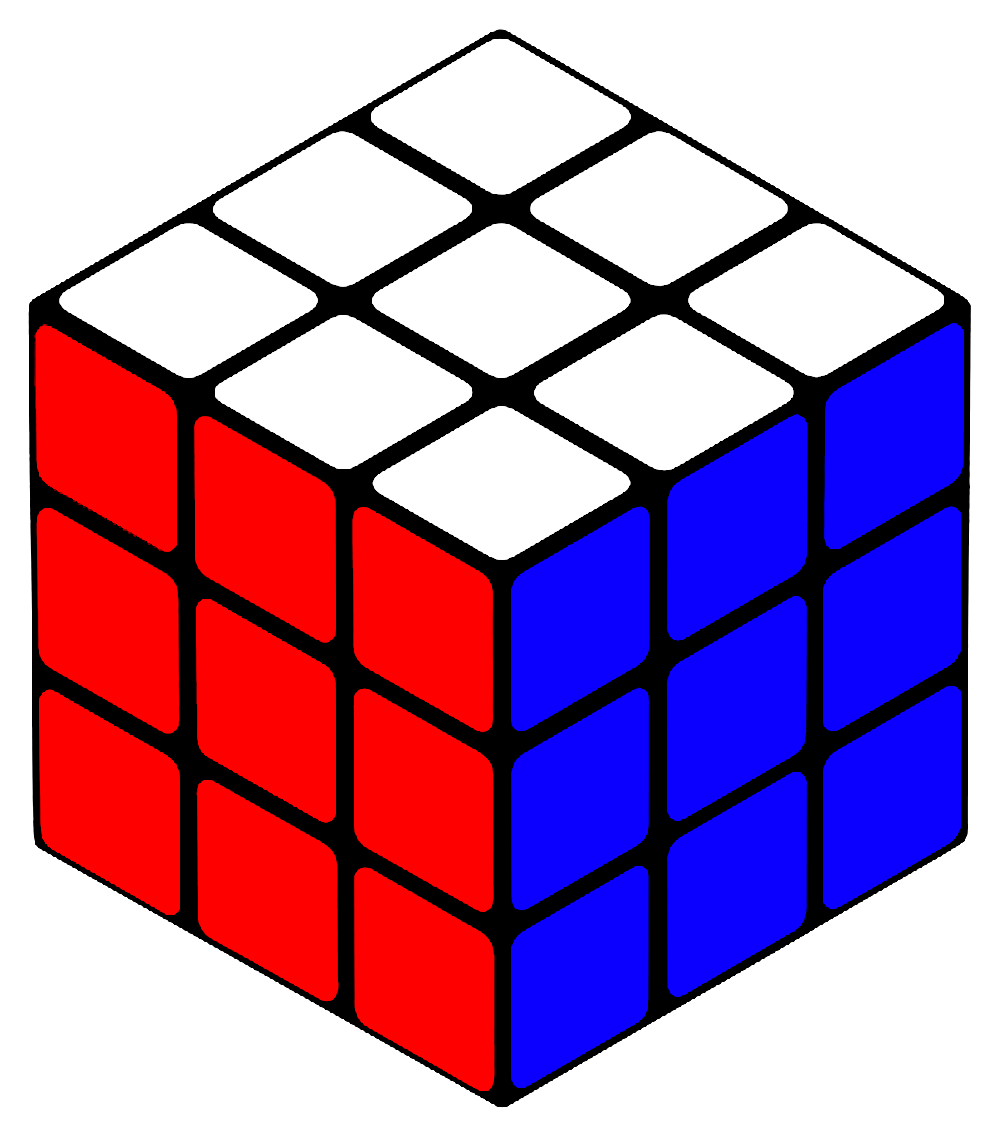
\includegraphics[scale=0.09]{3x3solved.png}
\caption{3x3x3 Zauberwürfel \\ (links in ungelöstem und rechts in gelöstem Zustand (auch Grundstellung))}
\end{figure}

\subsubsection*{Definition der Tiefe:}
Anzahl der Züge, die der Würfel von dem gelösten Zustand entfernt ist, wenn man den optimalen Lösungsweg wählt. Beim gelösten Zustand haben alle Felder auf einer Seite die gleiche Farbe. Die Tiefe des tiefsten Falls: Wie viele Züge kann der Würfel maximal von der Lösung entfernt sein? \\
Ein Zug ist das Drehen einer einzelnen Seite in eine beliebige Richtung, auch eine $180^\circ$ Drehung.

\subsubsection*{Algorithmen}
Am 2x2x2 Zauberwürfel gibt es an sich 6 verschiedene Drehseiten: oben, unten, links, rechts, vorne und hinten. Da der Würfel aber nur aus 2 Ebenen besteht, entspricht eine Drehung der oberen Ebene nach rechts einer Drehung der unteren Ebene nach links. Somit betrachte ich nur die Drehseiten oben, rechts und vorne. \\
Jede dieser Seiten kann nach im und gegen den Uhrzeigersinn gedreht werden, außerdem kann auch um $180^\circ$ gedreht werden. Die Abkürzungen für die Züge sind folgende: \\
\\
\begin{tabular}{|c|c|}
\hline
Abkürzung & Beschreibung des Zugs \\
\hline
\hline
$U$ & Drehung der oberen Ebene im Uhrzeigersinn \\
\hline
$U'$ & Drehung der oberen Ebene gegen den Uhrzeigersinn \\
\hline
$U180$ & Drehung der oberen Ebene um $180^\circ$, also $U180= UU = U'U'$ \\
\hline
$R$ & Drehung der rechten Ebene im Uhrzeigersinn \\
\hline
$R'$ & Drehung der rechten Ebene gegen den Uhrzeigersinn \\
\hline
$R180$ & Drehung der rechten Ebene um $180^\circ$, also $R180= RR = R'R'$ \\
\hline
$F$ & Drehung der vorderen Ebene im Uhrzeigersinn \\
\hline
$F'$ & Drehung der vorderen Ebene gegen den Uhrzeigersinn \\
\hline
$F180$ & Drehung der vorderen Ebene um $180^\circ$, also $F180= FF = F'F'$ \\
\hline
\end{tabular} \\
\\
$D$ ist analog zu $U$, aber untere statt obere Ebene, $L$ ist analog zu $R$ aber linke statt rechte Ebene und $B$ ist analog zu $F$ aber hintere statt vordere Ebene. 

\newpage


\section{(Geplante) Untersuchungen und Untersuchungsmethoden}



\subsection*{Code schreiben, der die Tiefe eines 2x2x2 Zauberwüfel berechnet}

Ich werde die Tiefe eines Zauberwürfels mit einem Java-Programm berechnen. Dazu werde ich den Würfel als Array darstellen. Jeder Farbfläche ist ein fester Index des Array zugeordnet, der die Farbe der Fläche als String enthält. \\
\begin{figure}[h]
\centering
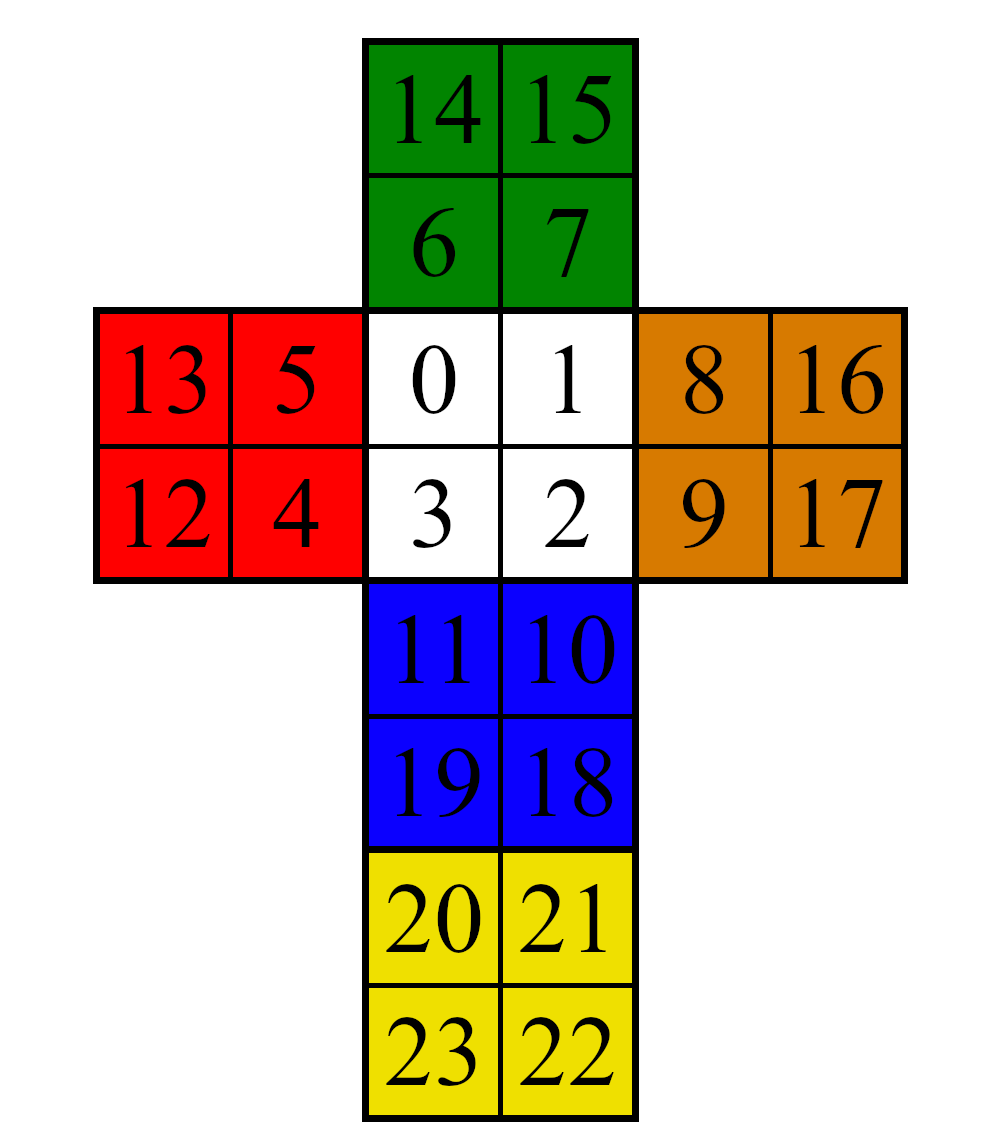
\includegraphics[scale=0.15]{2x2foldedout.png}
\caption{Zuordnung der Farbflächen zu den Indizes des Arrays.}
\end{figure}
\\
Das Array, das die Grundstellung repräsentiert, sieht beispielsweise folgendermaßen aus:
\begin{verbatim}
String [] solvedPosition =  {"white", "white", "white", "white", "red", 
"red", "green", "green", "orange", "orange", "blue", "blue", "red", 
"red", "green", "green", "orange", "orange", "blue", "blue", "yellow", 
"yellow", "yellow", "yellow"};
\end{verbatim}
Von dem gelösten Würfel ausgehend wird nun die Tiefe des tiefsten Falls gesucht. \\
Wenn der Würfel sich in einem Zustand der Tiefe $n$ befindet und ein Zug durchgeführt wird, muss einer der folgenden drei Fälle eintreten:
\begin{itemize}
	\item Die Tiefe der neuen Position ist $n+1$, der Würfel ist also einen Zug mehr von der Lösung entfernt.
	\item Die Tiefe der neuen Position ist die der alten, also $n+1$.
	\item Die Tiefe der neuen Positionen ist $n-1$, die Würfelposition ist also näher an der Lösung.
\end{itemize}
\begin{figure}[h]
\centering
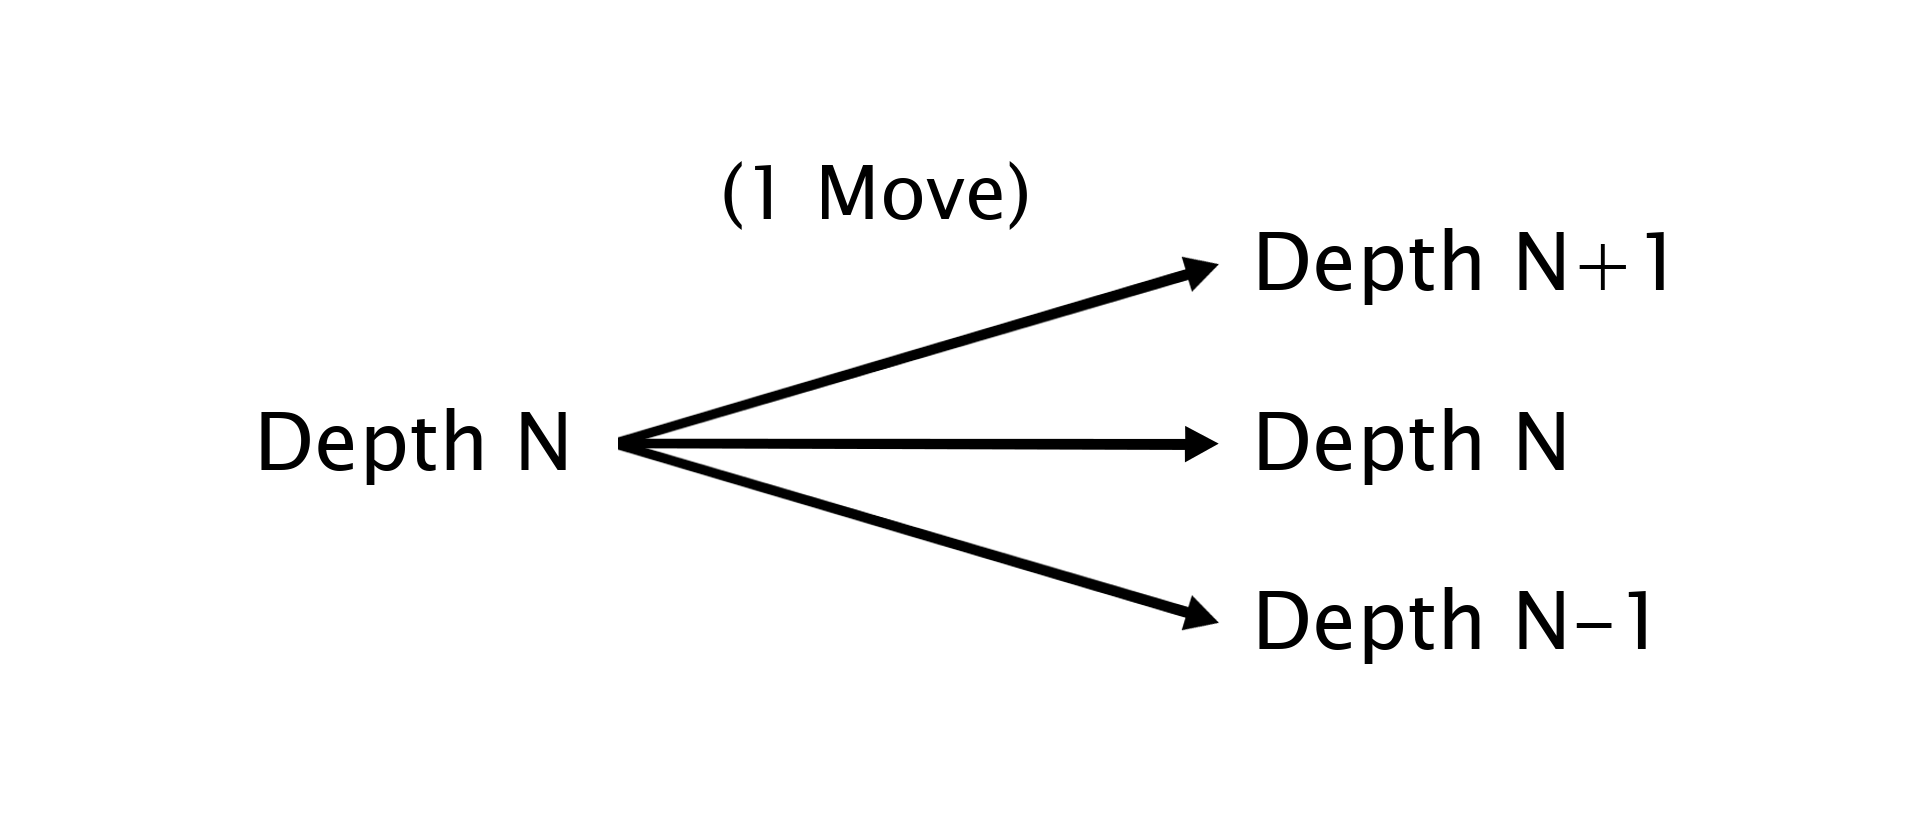
\includegraphics[scale=0.19]{graphDepth.png}
\end{figure}
Die Tiefe kann nicht negativ sein. Wenn man in einem Zustand der Tiefe $0$ einen Zug macht, hat der Würfel im Folgezustand immer die Tiefe 1. \\
Wenn man die maximale Tiefe $n_max$ erreicht hat, können die Folgezustände nur noch die Tiefe $n_{max}$ und $n_{max} -1$ haben. 
\begin{figure}[h]
\centering
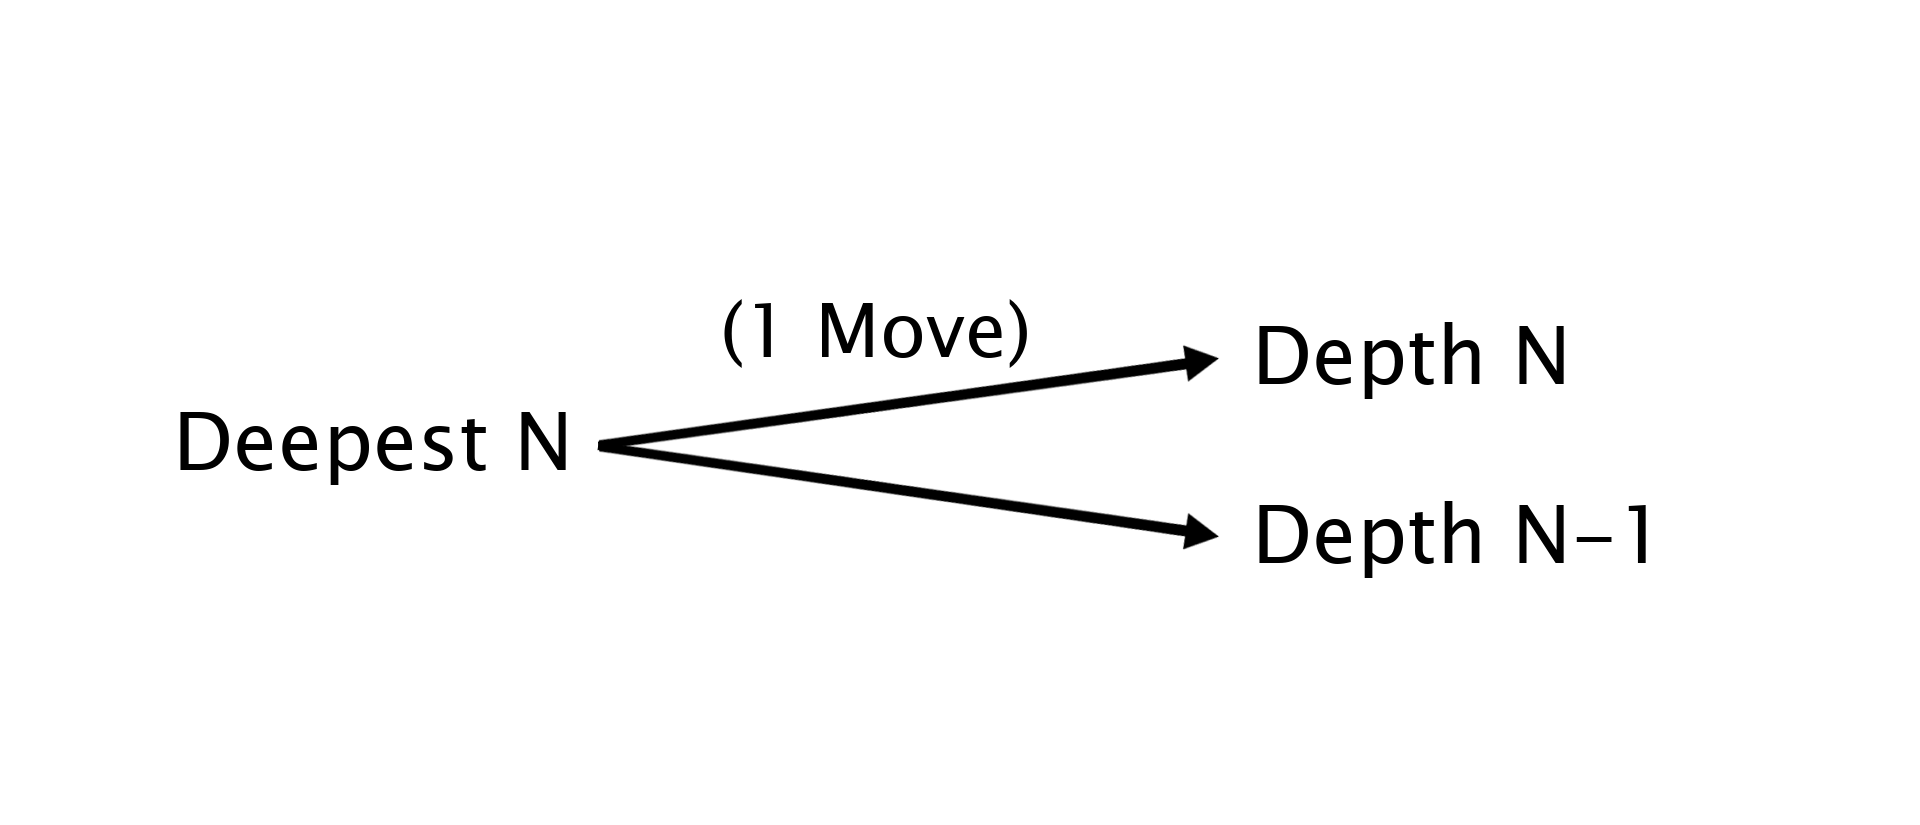
\includegraphics[scale=0.2]{graphDepthN.png}
\end{figure}
\\
Die möglichen Züge werden als einzelne Methoden implementiert (z.B. die Vorderseite um $90^\circ$ nach rechts drehen:
\begin{verbatim}
private static final int AMOUNT_FIELDS = 24;

    // Front um 90 Grad im Uhrzeigersinn (nach rechts) drehen
    public static String[] front (String [] currentPosition){
        String [] newPosition = new String[24];
        for (int i = 0; i < AMOUNT_FIELDS; i++){
            if (i < 2 || (i > 4 && i < 8) || (i > 12 && i < 17) || i > 21) {
                newPosition[i] = currentPosition[i];
            }
        }

        newPosition[2] = currentPosition[4];
        newPosition[3] = currentPosition[12];
        newPosition[4] = currentPosition[20];
        newPosition[9] = currentPosition[3];
        newPosition[10] = currentPosition[11];
        newPosition[11] = currentPosition[19];
        newPosition[12] = currentPosition[21];
        newPosition[17] = currentPosition[2];
        newPosition[18] = currentPosition[10];
        newPosition[19] = currentPosition[18];
        newPosition[20] = currentPosition[17];
        newPosition[21] = currentPosition[9];

        return newPosition;
    } ... }
\end{verbatim} \\
Bei der Implementierung der Züge werden die Züge $F, R, U$ implementiert und alle anderen lassen sich dadurch umsetzen. Zum Beispiel gilt $F' = FFF$ oder $U=F'$. \\
Mit diesen Methoden kann dann berechnet werden, welche Position welche Tiefe hat und so der Zustand mit der maximalen Tiefe errechnet werden.


\newpage 
\subsection*{Darstellung des 2x2x2 Zauberwüfels mit dem mathemtischen Konstrukt der Gruppe}
Definition einer kommutativen Gruppe $(G, \circ)$ (auch abelsche Gruppe):
\begin{itemize}
\item Abgeschlossenheit: $\forall a,b \in G.(a \circ b) \in G $
\item Assoziativität: $\forall a,b,c \in G.(a \circ b) \circ c = a \circ (b \circ c)$
\item Existenz eines neutralen Elements $n$: $\forall a \in G, \exists n \in G.n \circ a = a \circ n = a$ 
\item Existenz eines inversen Elements $a^{-1}$: $\forall a \in G, \exists a^{-1} \in G. a \circ a^{-1} = a^{-1} \circ a = n$ 
\item Kommutaivität: $\forall a,b \in G.a \circ b = b \circ a$
\end{itemize}
Die Gruppe des 2x2x2 Würfels nenne ich $(G_{2x2x2}, \circ)$. \\
\\
Sei $F_{Flaechen}$ die Menge aller Farbflächen, also $|F_{Flaechen}|=24$ mit $F_{Flaechen} = \lbrace 0, 2, ..., 23\rbrace$.
\\
\begin{figure}[h]
\centering
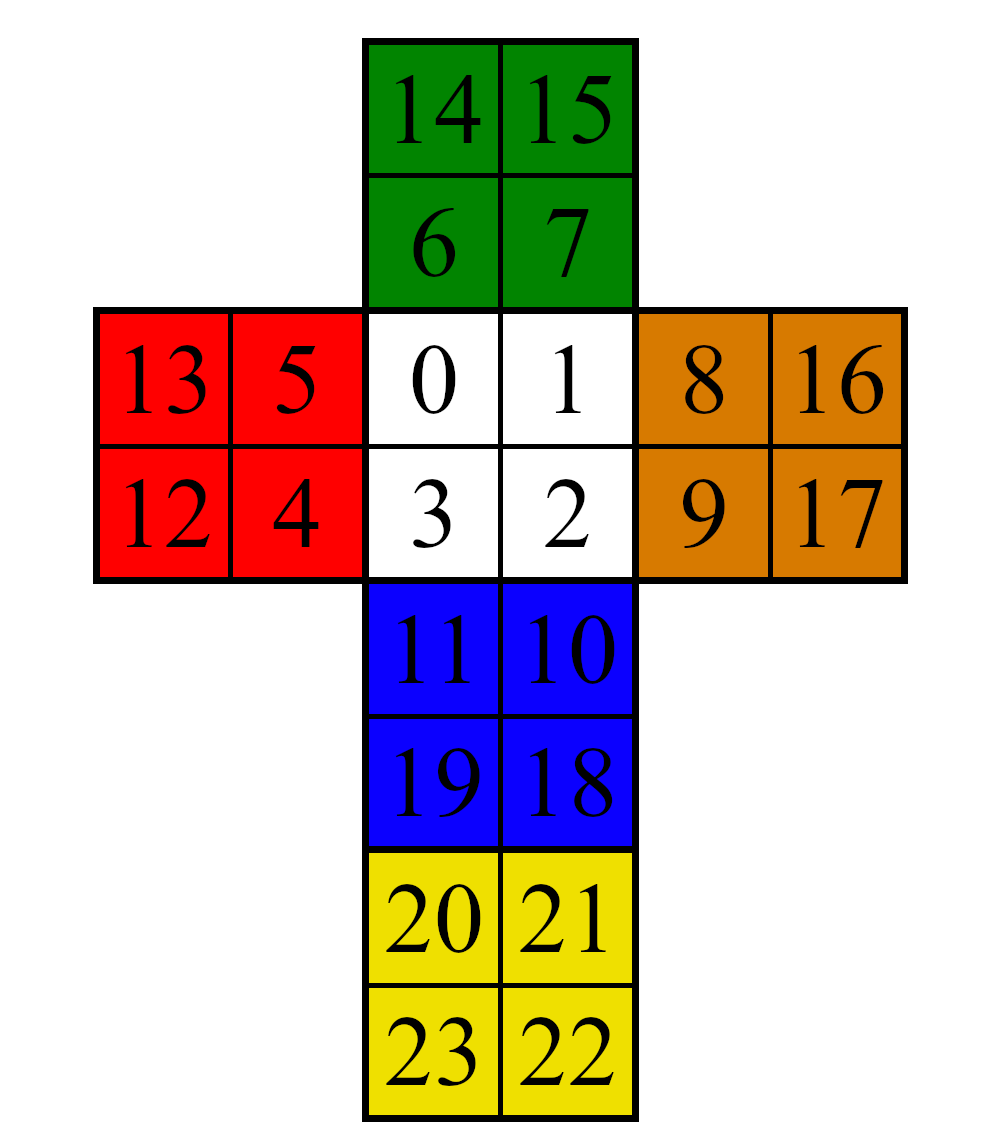
\includegraphics[scale=0.1]{2x2foldedout.png}
\end{figure}
\\
Die sechs Basiszüge sind $U, R, F, D, L, B$. Die Züge $D, L, B$ lassen sich durch Verknüpfungen von $U, R, F$ darstellen: \\ 
$D = U', D' = U, U' = UUU, DD = U'U',$ usw. \\
$R, F$ analog - Es lassen sich also alle Züge aus $U, R, F$ abbilden. \\
\\
\textbf{Gruppeneigenschaften von $(G_{2x2x2}, \circ)$:} \\
\\
Die Verknüpfung $\circ$ auf $G_{2x2x2}$ ist nicht kommutativ, da beispielsweise $F \circ U \neq U \circ F$.
So sieht der Würfel nach Anwendung der Züge \glqq Up nach Front anwenden\grqq ($F \circ U$) bzw \glqq Front nach Up anwenden\grqq ($U \circ F$) aus: \\
\begin{figure}[h]
\centering
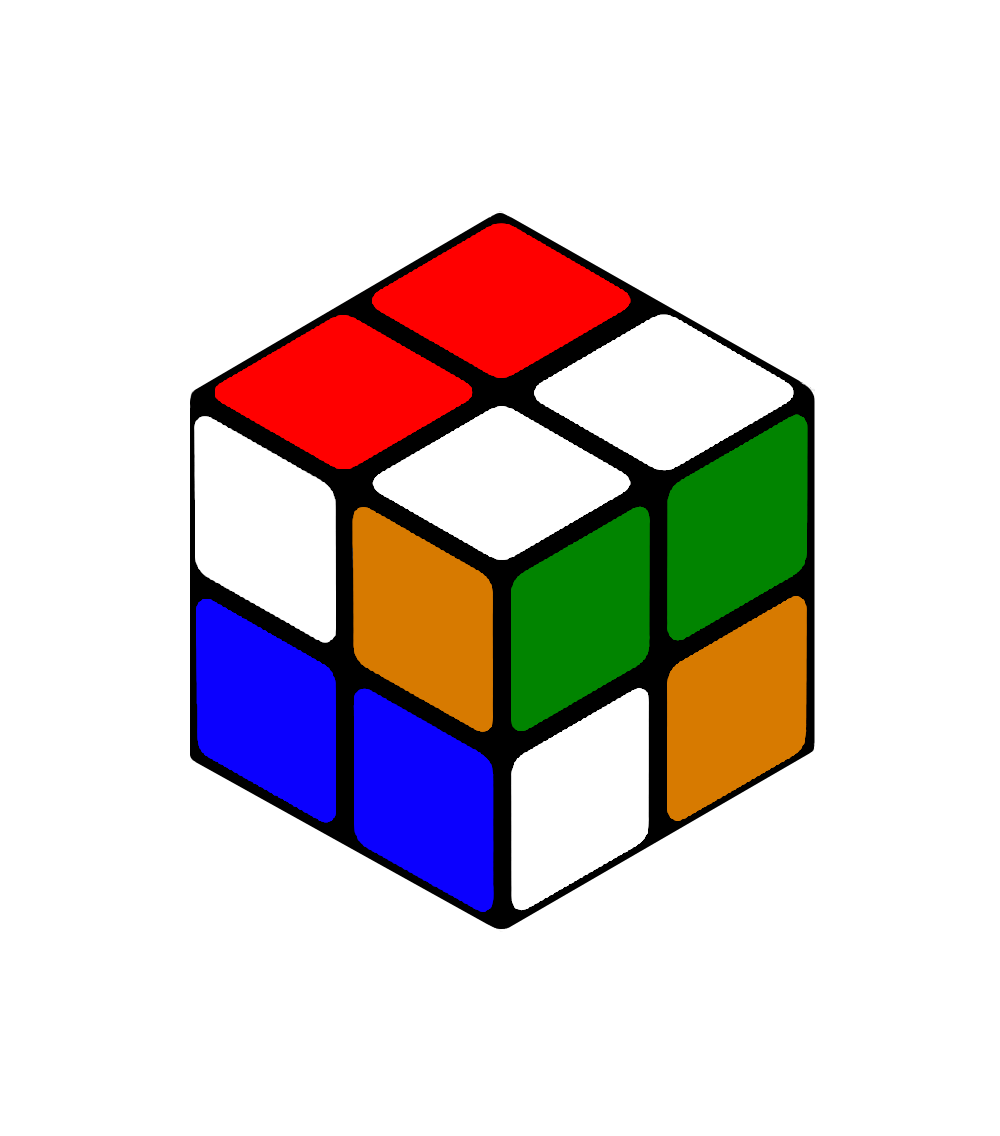
\includegraphics[scale=0.1]{UpAfterFront.png}
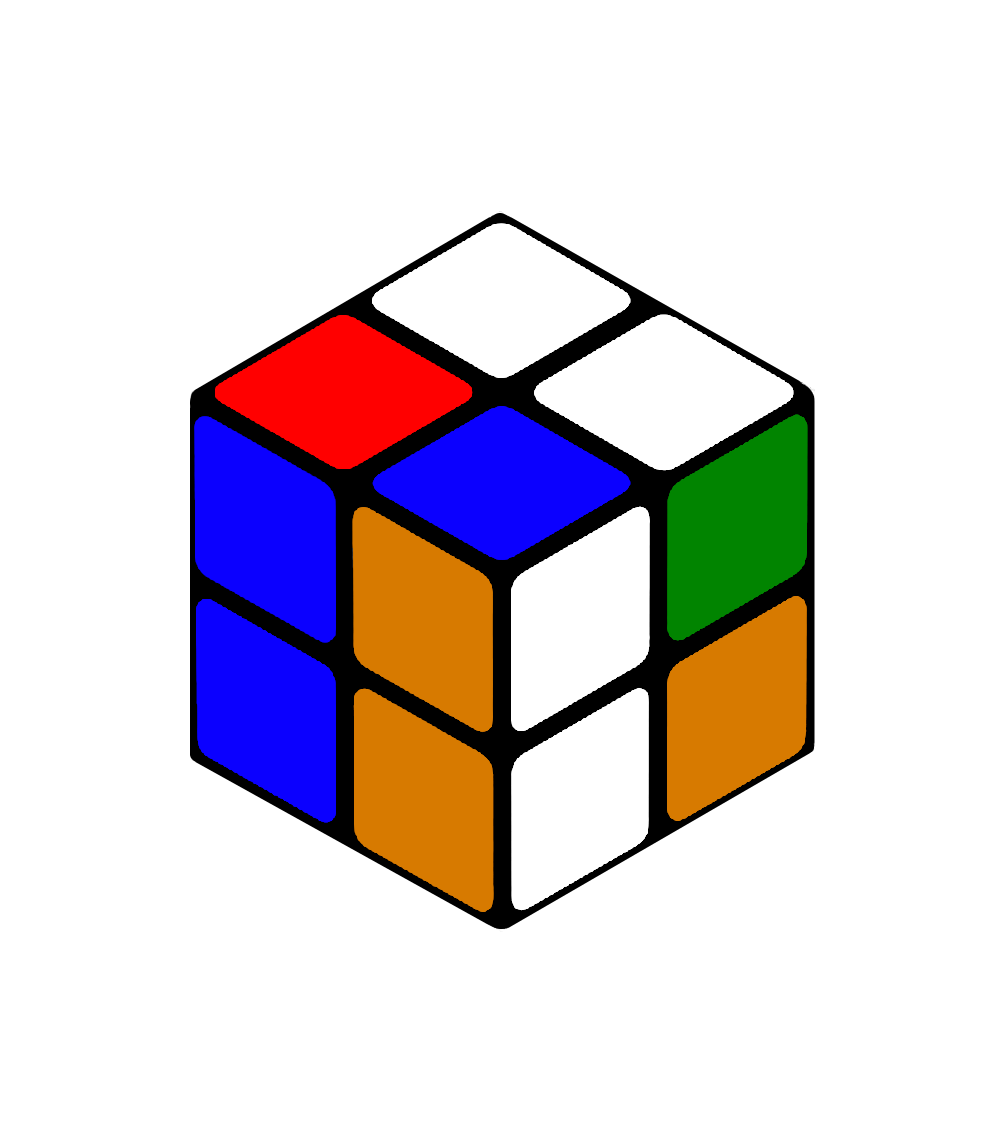
\includegraphics[scale=0.1]{FrontAfterUp.png}
\caption{links: $F \circ U$ und rechts: $U \circ F$}
\end{figure}
Die Gruppe $(G_{2x2x2}, \circ)$ ist also keine kommutative Gruppe. 
\\
\\
Neutrales Element: \\
Das neutrale Element nennt sich $id$, der Zustand des Würfels wird nicht verändert, indem kein Zug gemacht wird (oder beispielsweise vier mal der gleiche Zug: $FFFF = id$. \\
\\
Inverses Element: \\
Man kann zu jedem Zug $x \in \lbrace U, R, F, D, L, B \rbrace$ auch den passenden Zug $x' = xxx$ bilden. Das entspricht einer Rückdrehung und somit dem inversen Element. Beispielsweise $F \circ F' = id$. Umgekehrt funktioniert es genauso: $F' \circ F = id$. Das funktioniert für alle Elemente aus der Menge der Züge $Z=\lbrace U, R, F, D, L, B \rbrace$.
\begin{figure}[h]
\centering
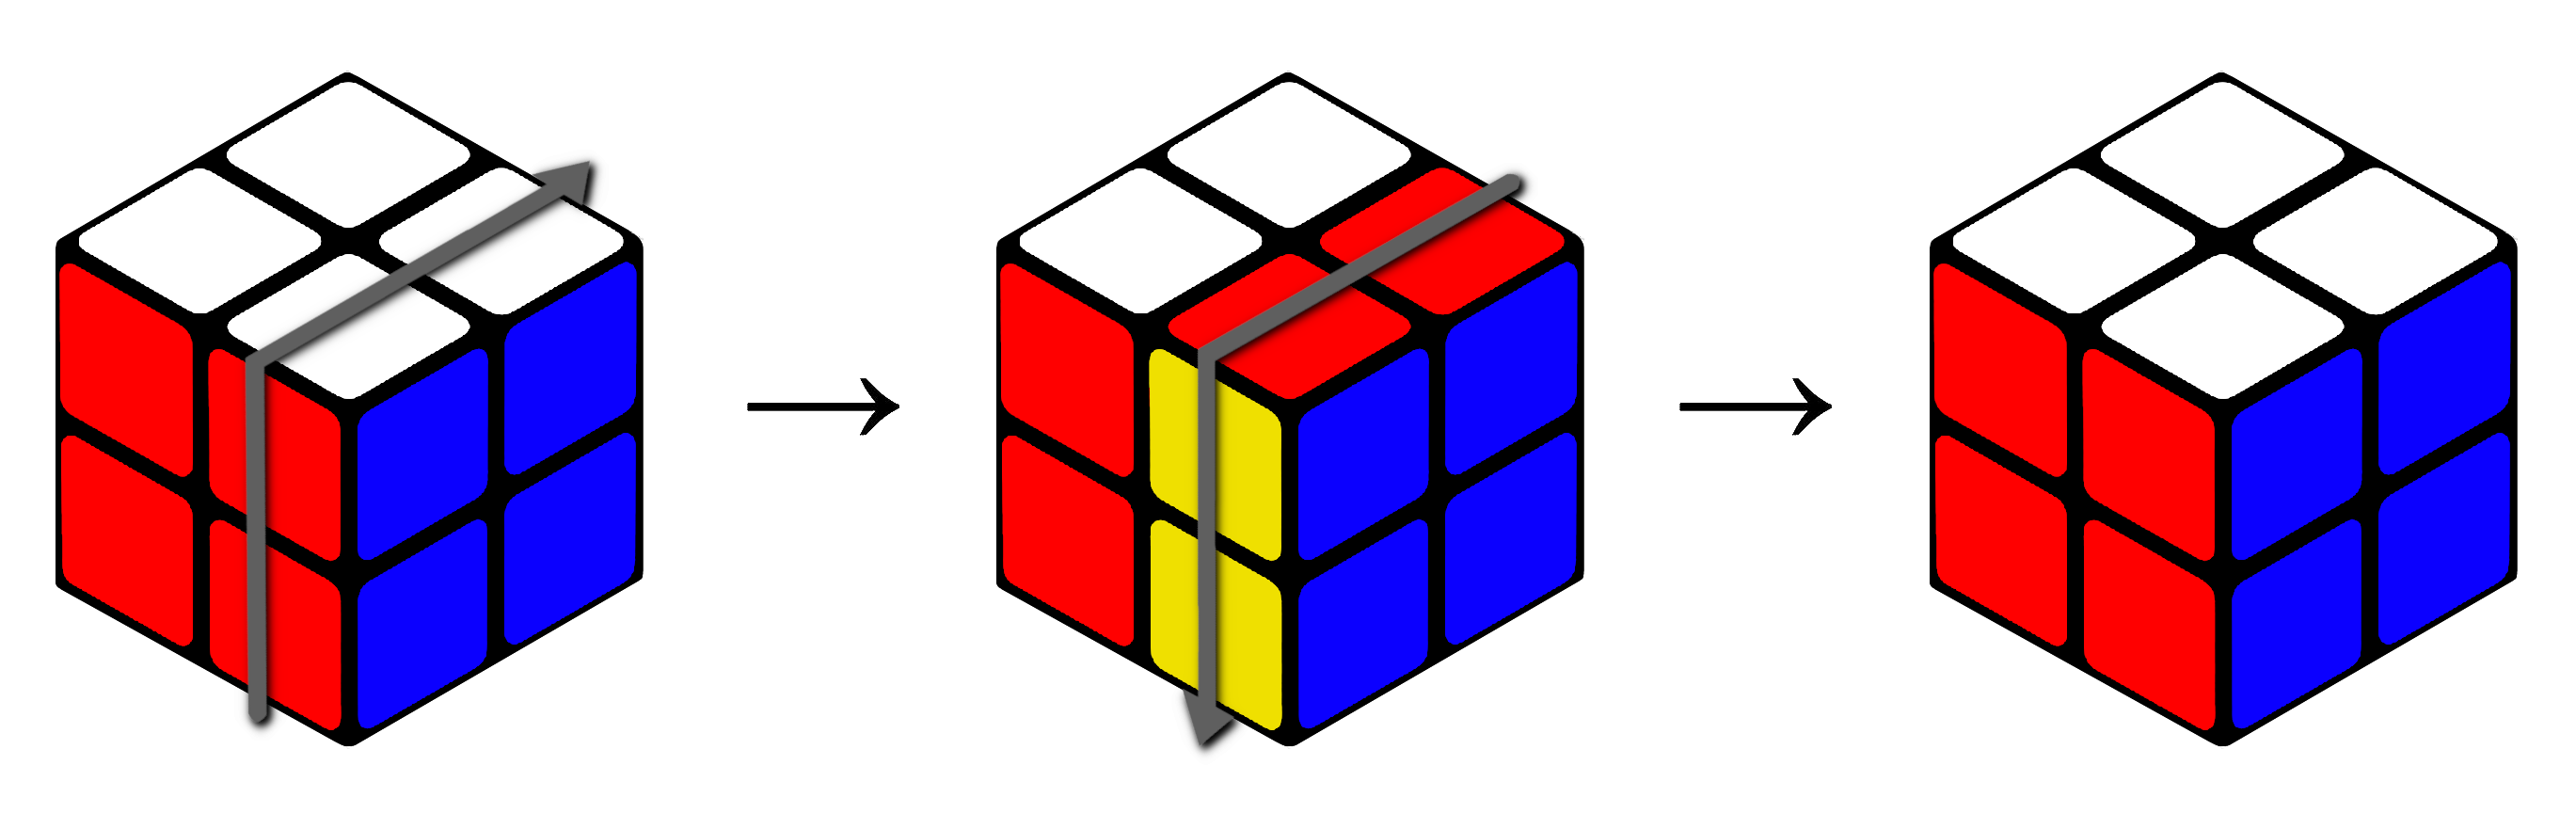
\includegraphics[scale=0.07]{inverses.png}
\caption{$F \circ F' = id$}
\end{figure}
\\
Assoziativität: \\
$(X_1 \circ X_2) \circ X_3$ also $X_2$ nach $X_1$ anwenden und dann $X_3$, das enstrpicht also $X_1, X_2, X_3$.
$X_1 \circ (X_2 \circ X_3) = $ also $X_3$ nach $X_2$ nach $X_1$, das entspricht $X_1, X_2, X_3$.
Somit ist $\circ$ assoziativ. \\
\\
\\
\textbf{Permutationen: } \\
\begin{figure}[h]
\centering
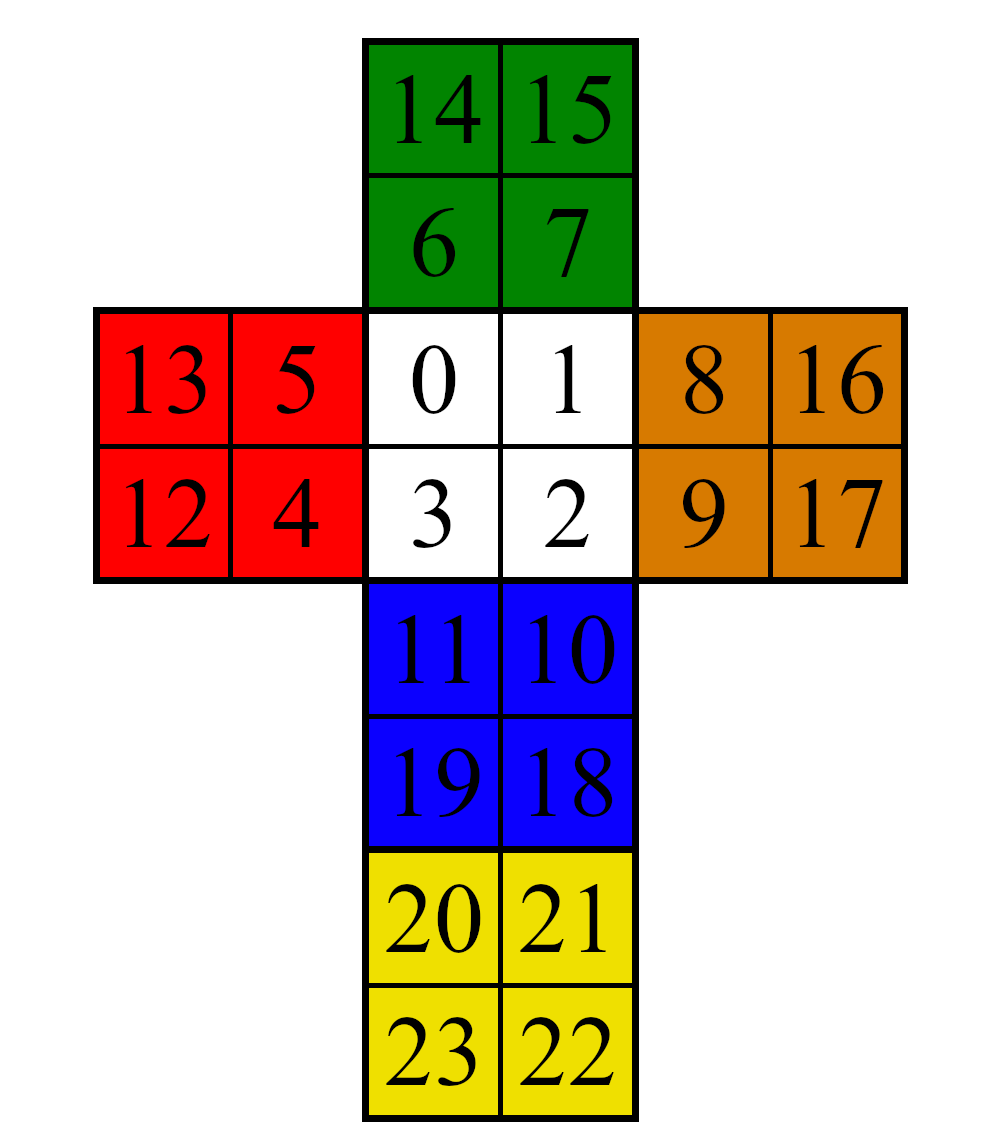
\includegraphics[scale=0.1]{2x2foldedout.png}
\end{figure}
\\
Vertauschung bei einer Drehung: \\
Wenn man nun den Zug $F$ ausführt, also eine Drehung der blauen Ebene (der Vorderseite) um $90^\circ$ nach rechts, treten folgende Vertauschungen auf: \\ \\
\begin{tabular}{|c|c|c|c|c|c|c|c|c|c|c|c|c|}
\hline
Grundstellung & \color{gray}{0} & \color{gray}{1} & \color{gray}{2} & \color{gray}{3} & \color{red}{4} & \color{red}{5} & \color{ForestGreen}{6} & \color{ForestGreen}{7} & \color{orange}{8} & \color{orange}{9} & \color{blue}{10} & \color{blue}{11} \\
\hline
neuer Zustand & \color{gray}{0} & \color{gray}{1} & \color{red}{4} & \color{red}{12} & 20 & \color{red}{5} & \color{ForestGreen}{6} & \color{ForestGreen}{7} & \color{orange}{8} & \color{gray}{3} & \color{blue}{11} & \color{blue}{19} \\
\hline
\hline
Grundstellung & \color{red}{12} & \color{red}{13} & \color{ForestGreen}{14} & \color{ForestGreen}{15} & \color{orange}{16} & \color{orange}{17} & \color{blue}{18} & \color{blue}{19} & 20 & 21 & 22 & 23 \\
\hline
neuer Zustand & 21 & \color{red}{13} & \color{ForestGreen}{14} & \color{ForestGreen}{15} & \color{orange}{16} & \color{gray}{2} & \color{blue}{10} & \color{blue}{19} & \color{orange}{17} & \color{orange}{9} & 22 & 23\\
\hline
\end{tabular} \\
Farberklärung: \color{gray}{weiß}, \color{blue}{blau}, \color{ForestGreen}{grün}, \color{orange}{orange}, \color{black}{gelb}, \color{red}{rot}\\
\\
\color{black}{An} diesem Beispiel sieht man, dass die Felder, die vor dem Zug blau waren, auch danach alle noch blau sind. Es befinden sich allerdings andere Farbflächen an ihrer Stelle, da ja die vordere (blaue) Fläche gedreht wurde. \\
\\
Die Permutation für $F$ schreibt man auch so auf: \\
$\footnotesize
\sigma_F=
\left( \begin{array}{cccccccccccccccccccccccc}
0 & 1 & 2 & 3 & 4 & 5 & 6 & 7 & 8 & 9 & 10 & 11 & 12 & 13 & 14 & 15 & 16 & 17 &  18 & 19 & 20 & 21 &22 & 23 \\                                           
0 & 1 & 4 & 12 & 20 & 5 & 6 & 7 & 8 & 3 & 11 & 19 & 21 & 13 & 14 & 15 & 16 & 2 & 10 & 19 & 9 & 22 & 17 & 23 \\
\end{array}\right)$
Also: $\sigma_F(0) =0, \sigma_F(1)= 1, \sigma_F(2)=4, \sigma_F(3)=12,...$ \\
\\
Die Menge aller Permutationen enthält $id$, für eine Permutation, die den Zustand nicht verändern, also: \\
$\footnotesize
\sigma_{id}=
\left( \begin{array}{cccccccccccccccccccccccc}
0 & 1 & 2 & 3 & 4 & 5 & 6 & 7 & 8 & 9 & 10 & 11 & 12 & 13 & 14 & 15 & 16 & 17 &  18 & 19 & 20 & 21 &22 & 23 \\                                           
0 & 1 & 2 & 3 & 4 & 5 & 6 & 7 & 8 & 9 & 10 & 11 & 12 & 13 & 14 & 15 & 16 & 17 &  18 & 19 & 20 & 21 &22 & 23 \\                                           
\end{array}\right)$
\\
\\
Außerdem ist für jeden Zug eine Permutation vorhanden. Die Menge aller Permutationen ist also $M_{perm} = \lbrace id, \sigma_U, \sigma_R, \sigma_F, \sigma_D, \sigma_L, \sigma_B \rbrace$


%Definition einer Permutationsgruppe $(G, \cdot)$: \\
%(Gruppe von Permutationen einer endlichen Menge F (Menge der Farbflächen).)\\
%Sei $G, \cdot$ eine Gruppe mit neutralem Element $e$:
%\begin{itemize}
%\item F ist eine endliche Menge.
%\item $G$ operiert auf $F$: Es existiert eine Abbildung $G \times M \rightarrow M, (g,m) \mapsto g \circ m \in M$, %für die gilt $\forall m \in M, g,h \in G.e \circ m =m, (g \cdot h) \circ m = g \circ (h \circ m)$
%\item Operation $\circ$ ist treu, es gilt: Ist $g \circ m = h \circ m.\forall m \in M$ dann folgt $g=h$. Gilt $g %\circ m = m$ dann folgt $g = e$.
%\end{itemize}


\subsection*{Übertragung der 3x3x3 Algorithmen auf den 2x2x2 Zauberwüfel}

Wird im Laufe der Arbeit noch erarbeitet. Zuerst muss aber die Darstellung in der Gruppentheorie (sowohl für den 3x3x3 Würfel als auch den 2x2x2 Qürfel fertig sein. Der Umfang dieses Teils steht in Abhängigkeit zu dem Umfang des Codes und der Darstellung in der Gruppentheorie. \\

\newpage


\section{Zeitplan}
Da aktuell die Klausuren wegen der Corona-Pandemie abgesagt bzw. verschoben wurden, kann ich den Zeitplan nicht anhand genauer Daten bilden, da der Anmeldezeitpunkt meiner Arbeit noch unklar ist. \\
Ich werde aber meine Vorgehensweise und die Inhalte hier genauer beschreiben. \\
Die Bearbeitungszeit einer Bachelorarbeit beträgt 4 Monate (ich werde hier mit etwa 17 Wochen rechnen). \\
Bis jetzt habe ich folgende Quellen genutzt (bzw. vor, diese für  meine Arbeit zu nutzen): Buch: Elementar(st)e Gruppentheorie von Tobias Glosauer (Springer Verlag), Magazin: Spektrum der Wissenschaft - Von Primzahlen zu Monstergruppen (Ausgabe 4.18) und diverse Internetseiten. Sebstverständlich werden die Quellen in meiner Arbeit korrekt angegeben. \\
Für die Einleitung und die Beschreibung des Aufbaus eines Zauberwürfels plane ich etwa eine Woche ein. \\
Für das Schreiben des Codes zwei Wochen, das Beschreiben des Codes sollte etwa eine weitere Woche in Anspruch nehmen. \\
Die Darstellung des 2x2x2 Würfels mit der Gruppentheorie plane ich für drei Wochen. \\
Um die 3x3x3 Algorithmen auf den 2x2x2 Würfel zu übertragen, muss sowohl die Darstellung des 2x2x2 als auch des 3x3x3 mit der Gruppentheorie oder in anderer (einheitlicher) Weise erfolgt sein - dafür plane ich weitere zwei Wochen ein. \\
Das Übertragen der 3x3x3 Algorithmen auf den 2x2x2 Würfel dauert dann noch weitere drei Wochen. \\
Dann plane ich für Quellenangaben, Formatierung, Grafiken und Schreiben noch zwei weitere Wochen ein. \\
Somit habe ich (hoffentlich) nicht zu knapp geplant und meine Bearbeitungszeit würde sich auf 14 Wochen betragen. Mit Rücksprachen, Anmerkungen, Kritik und Gegenlesung sollte die Arbeit in dem 17 Wochen Zeitrahmen zu schaffen sein. \\ 
Ich hoffe, es ist verständlich, dass ein Zeitplan im Vorraus nicht allzu genau werden kann. \\


\section{Abbildungen, Tabellen etc.}

Alle bisher verwendeteten Grafiken, Abbildungen und Tabellen habe ich selbst (mit GIMP oder LateX) erstellt, um Markennennungen zu vermeiden und eine einheitliche Darstellung zu gewährleisten.
Alle verwendeten Abbildungen: \\
\begin{figure}[h]
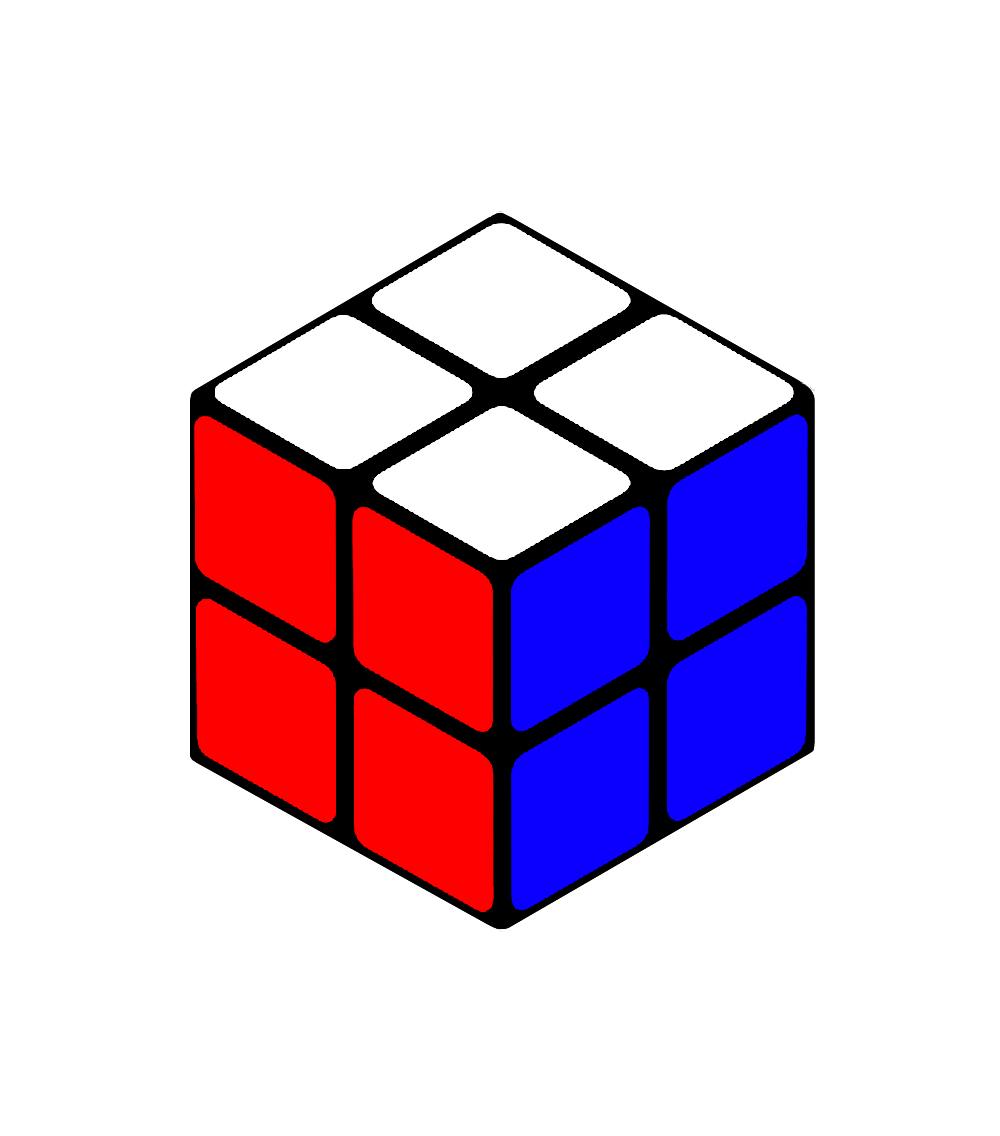
\includegraphics[scale=0.04]{2x2solved.png}
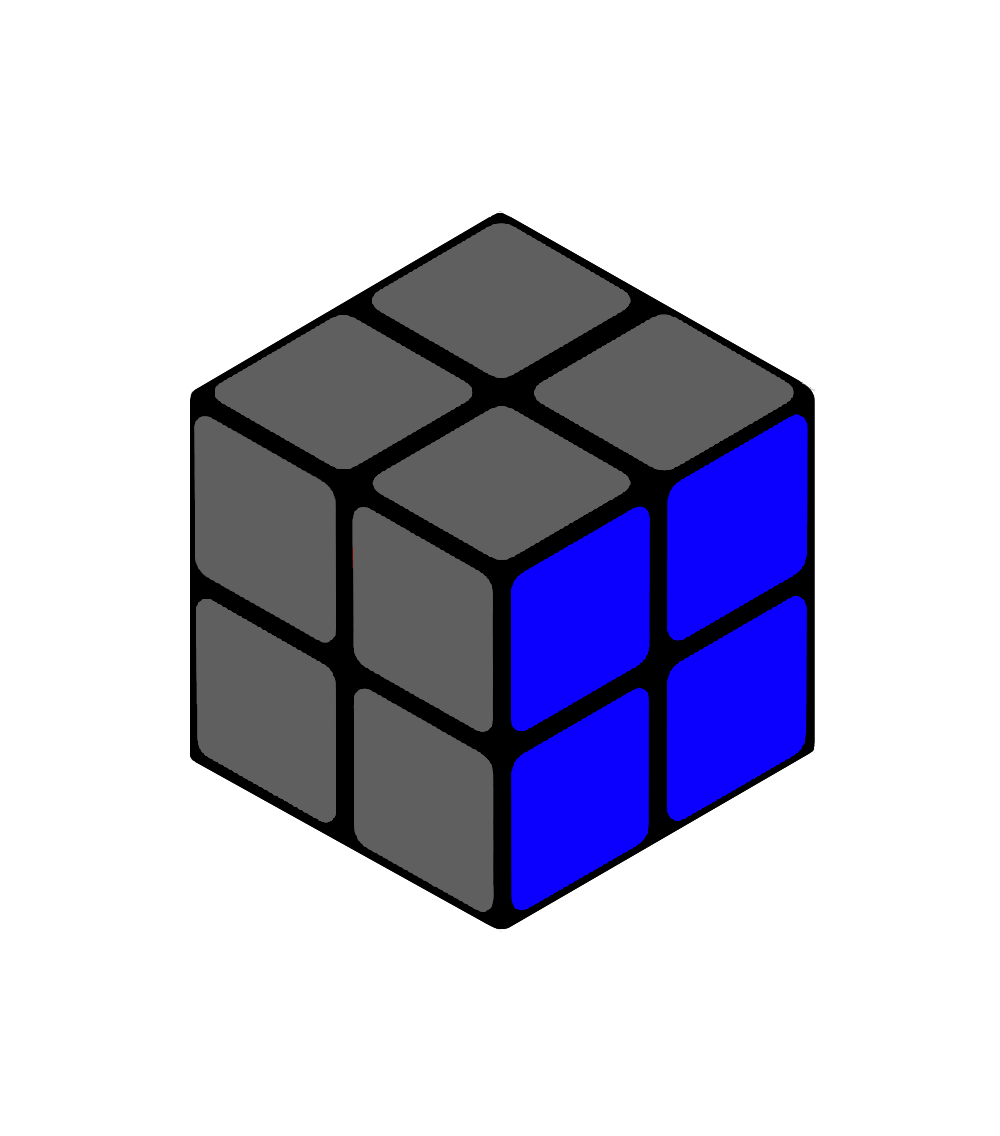
\includegraphics[scale=0.04]{2x2seite.png}
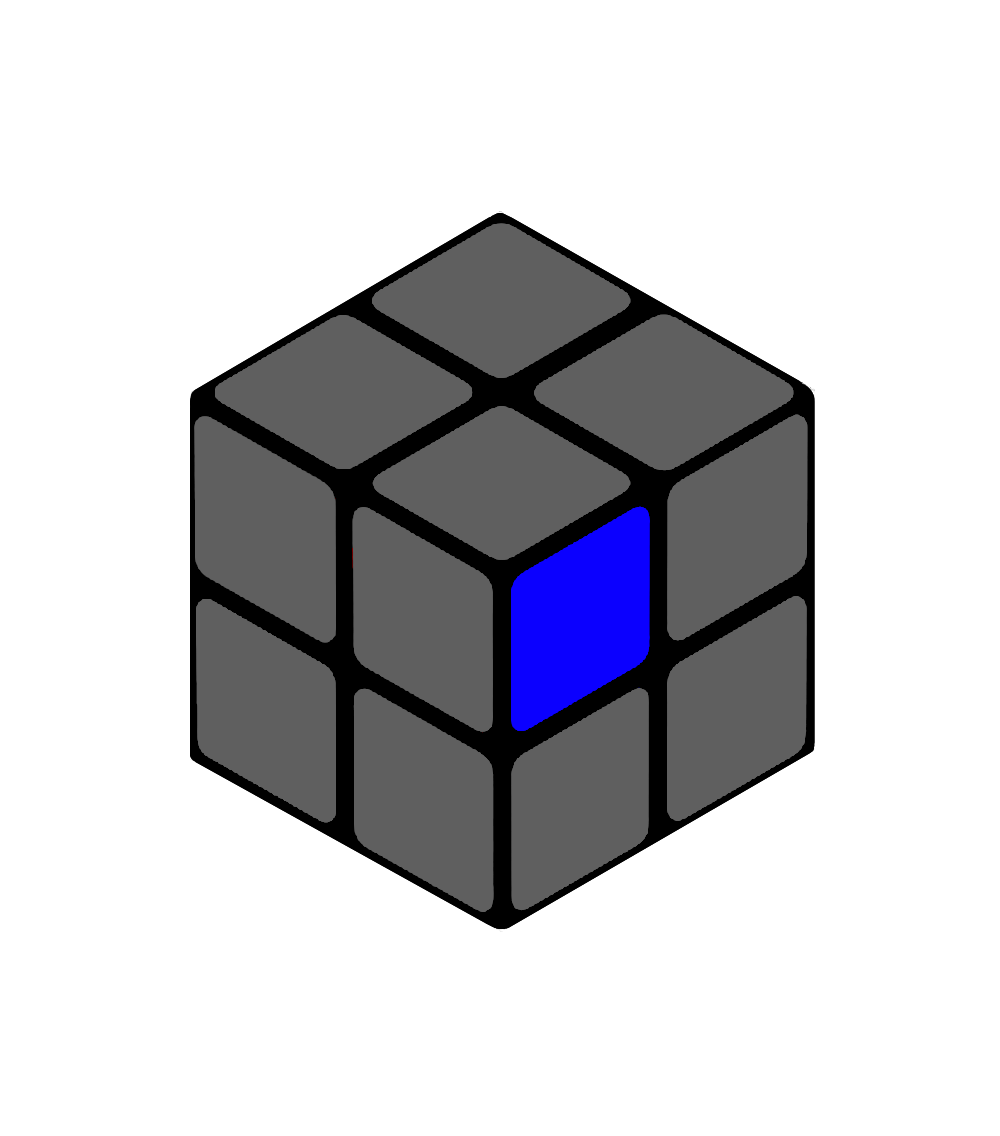
\includegraphics[scale=0.04]{2x2farbflaeche.png}
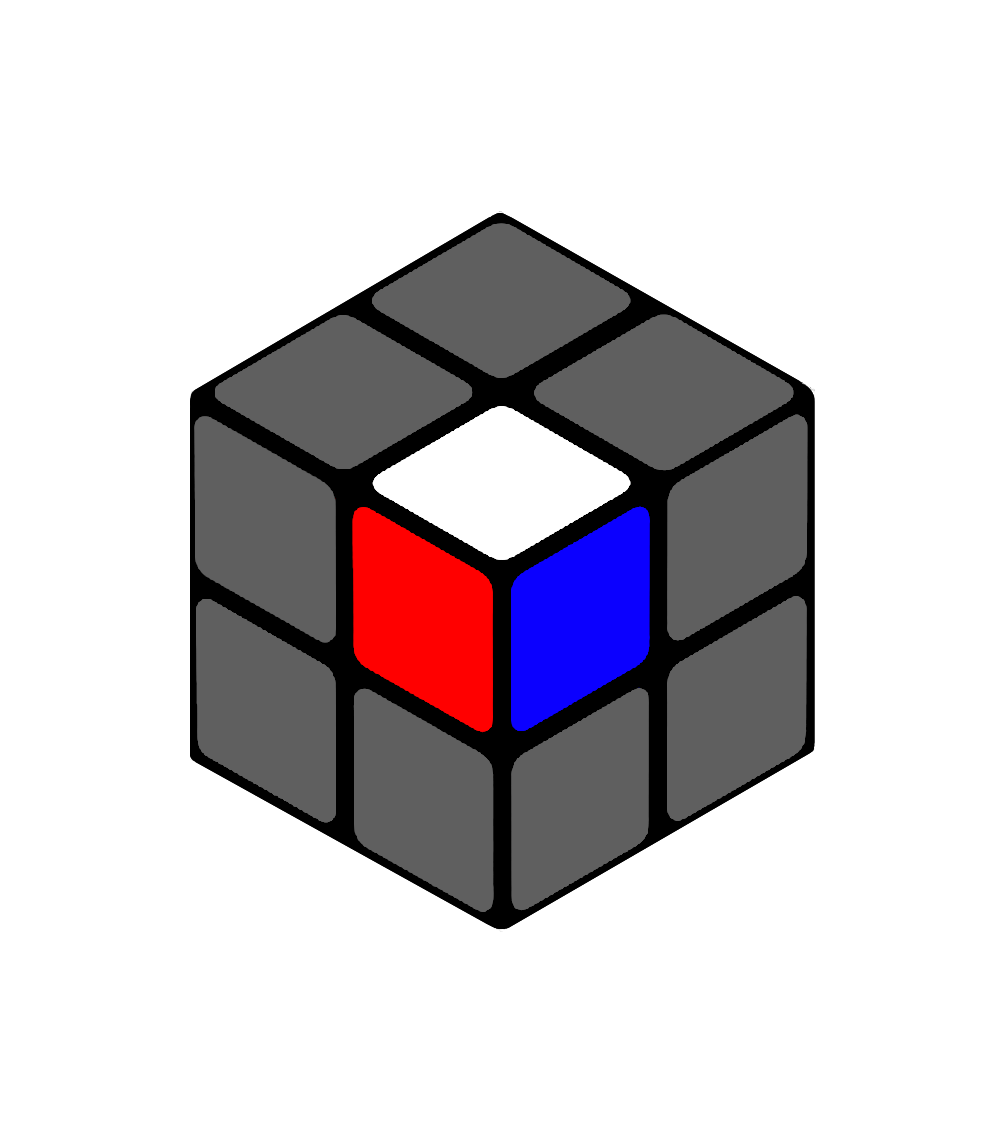
\includegraphics[scale=0.04]{2x2stein.png} 
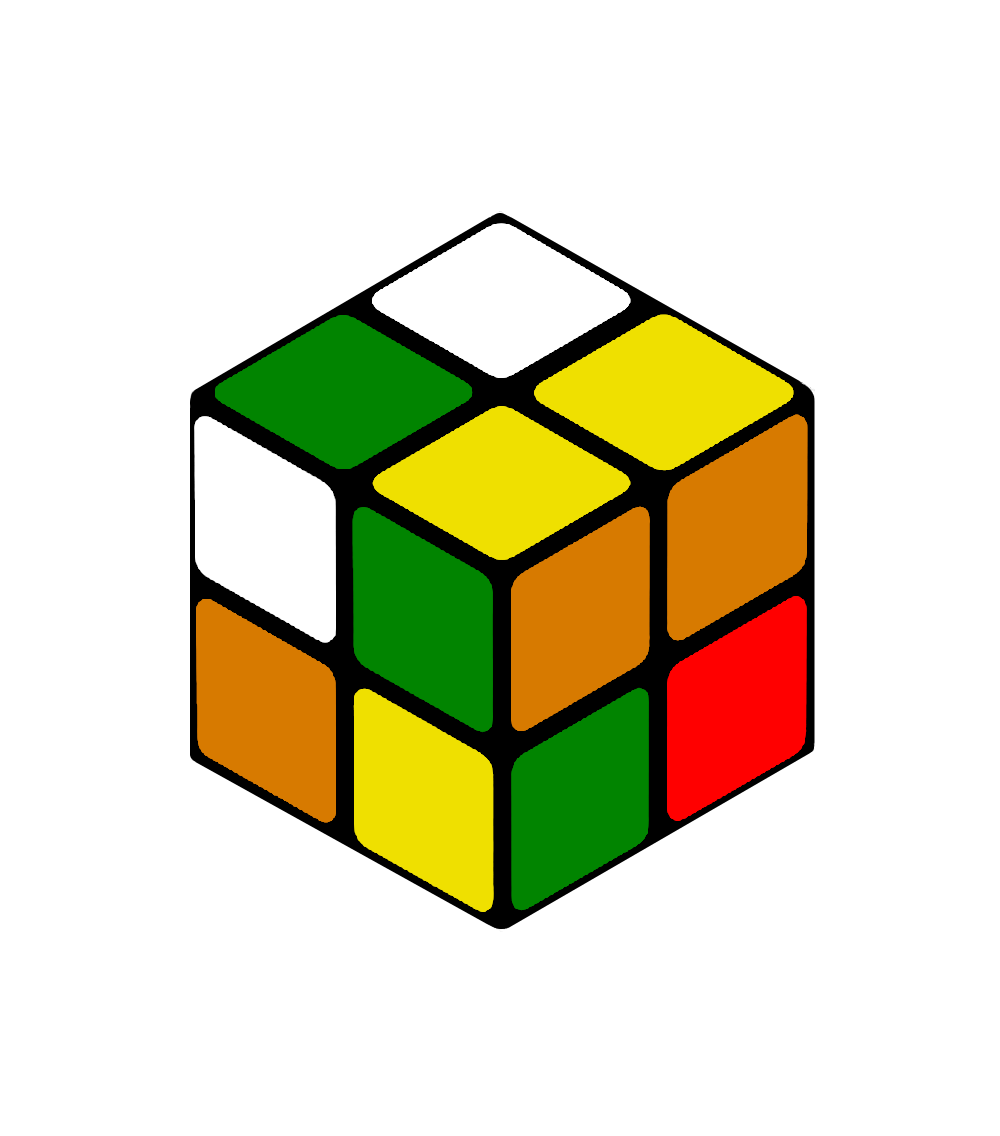
\includegraphics[scale=0.04]{2x2scrambled.png}
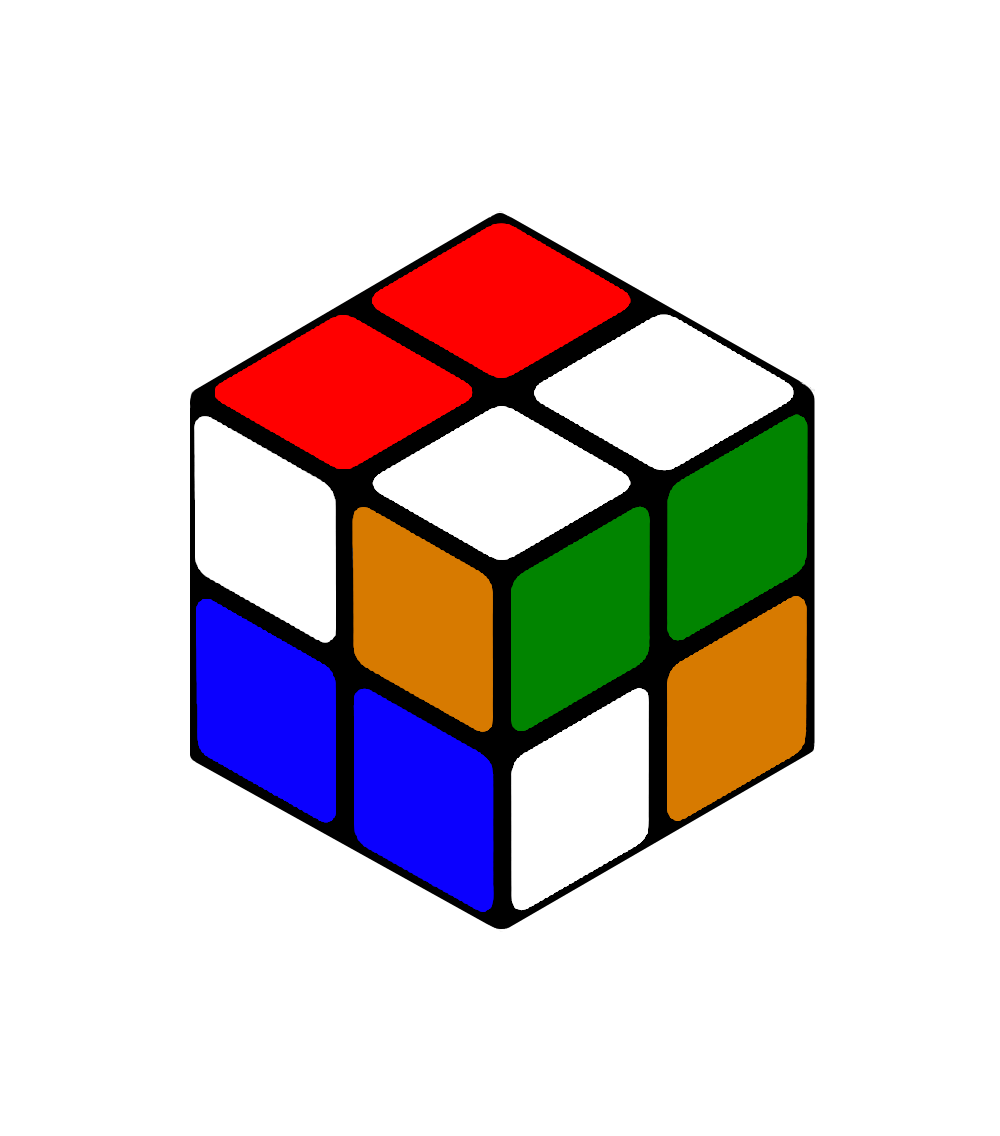
\includegraphics[scale=0.04]{UpAfterFront.png}
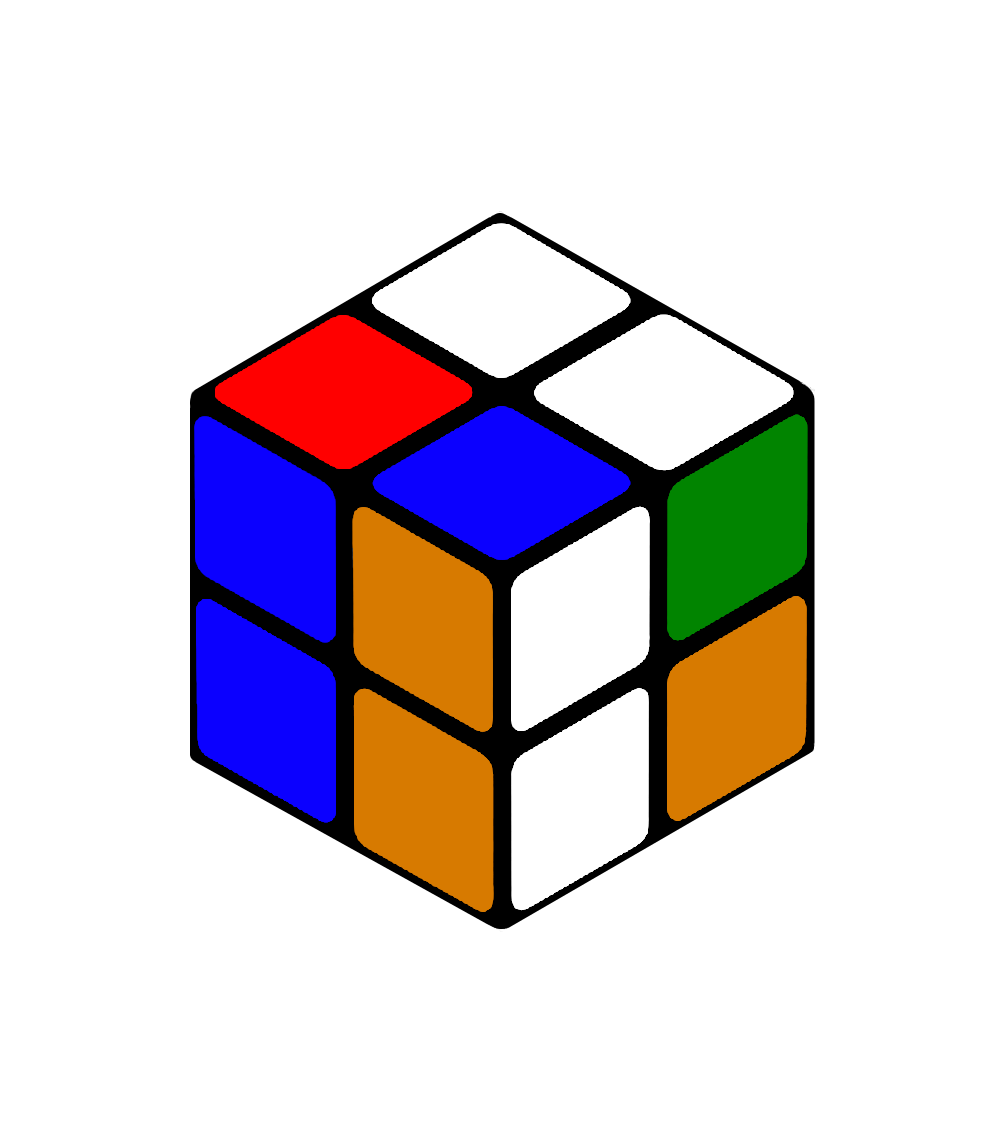
\includegraphics[scale=0.04]{FrontAfterUp.png}
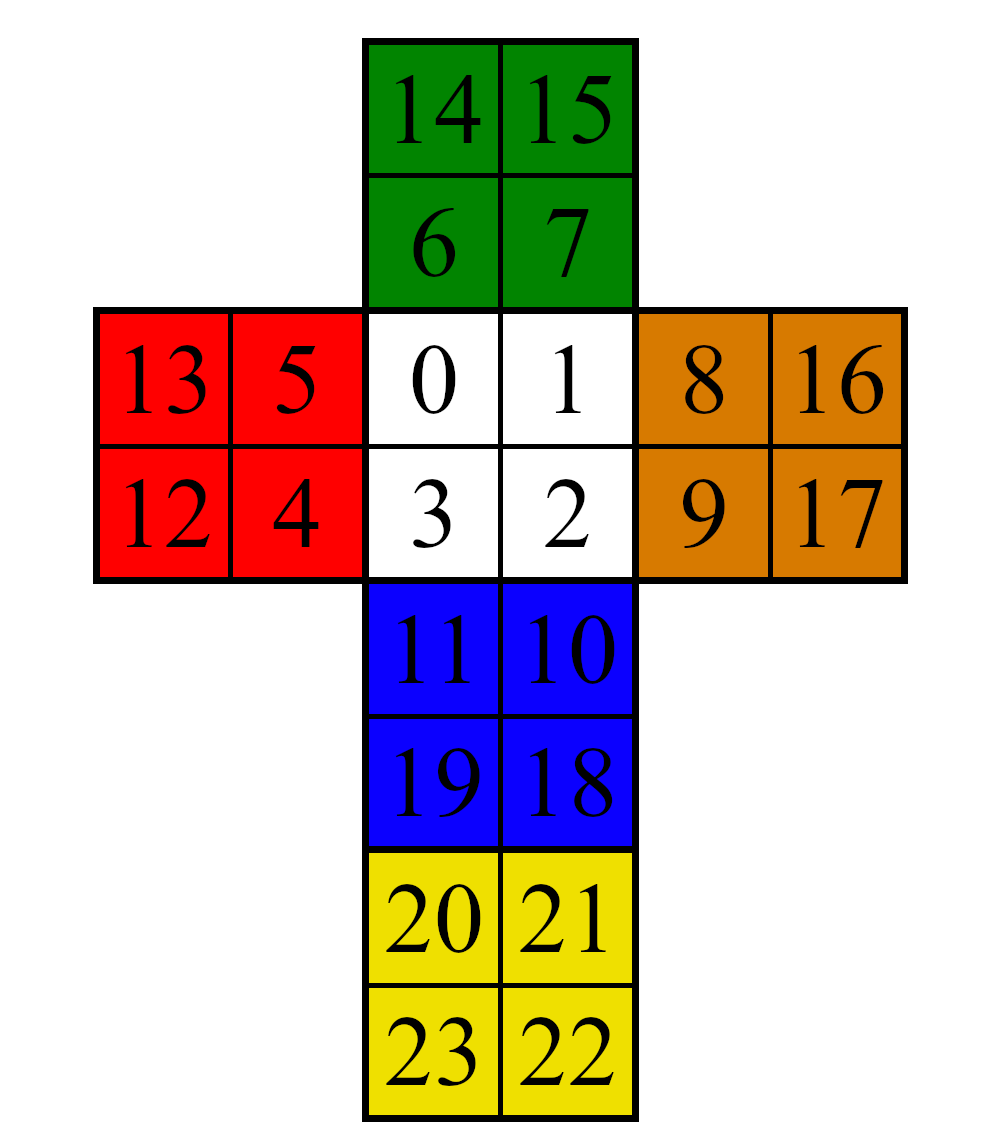
\includegraphics[scale=0.04]{2x2foldedout.png} \\
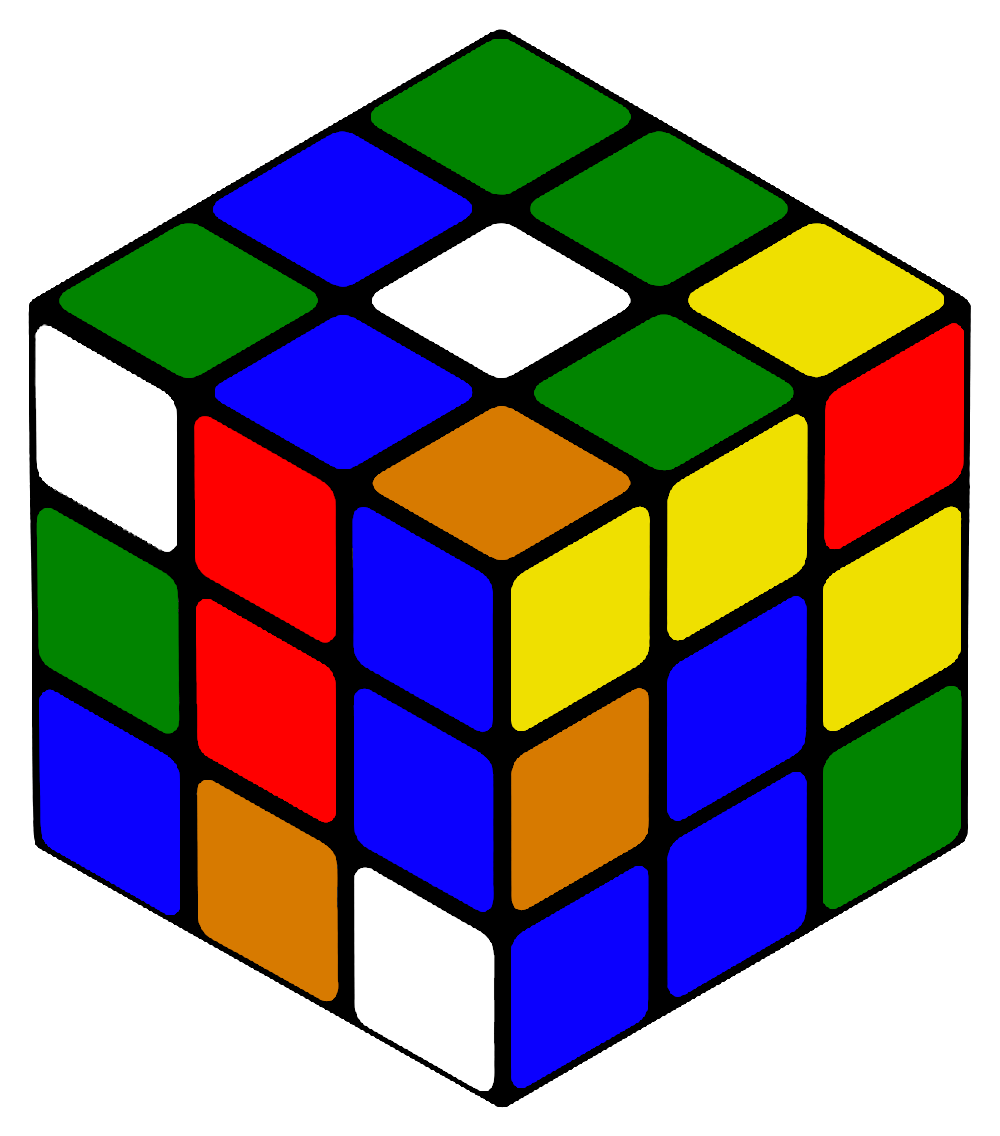
\includegraphics[scale=0.04]{3x3scrambled.png}
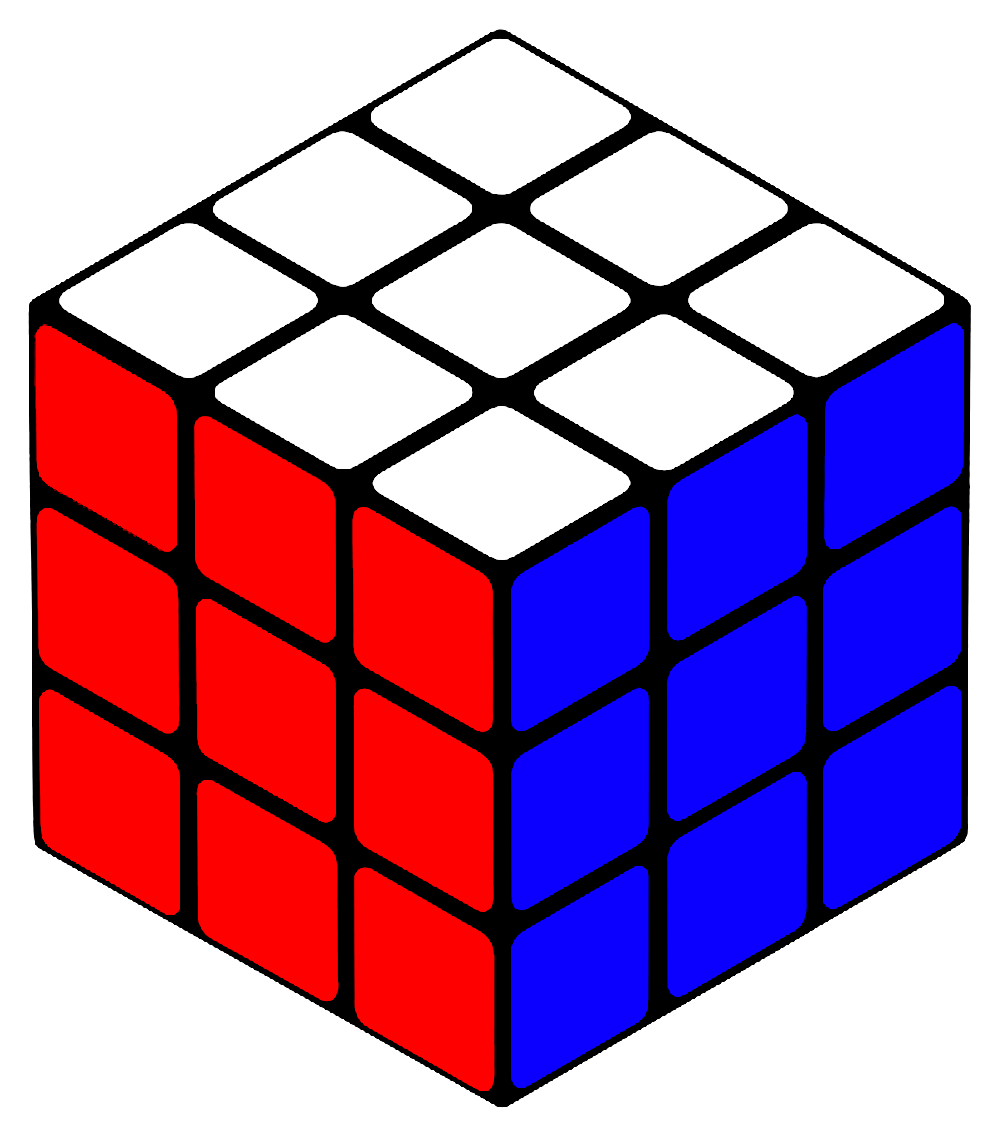
\includegraphics[scale=0.04]{3x3solved.png}
\end{figure}

\end{document}




